\documentclass{article}
\usepackage{tikz}
\usepackage{amsmath}
\usepackage{breqn}
\usepackage{amssymb}
\usepackage[ruled,vlined]{algorithm2e}
\begin{document}
	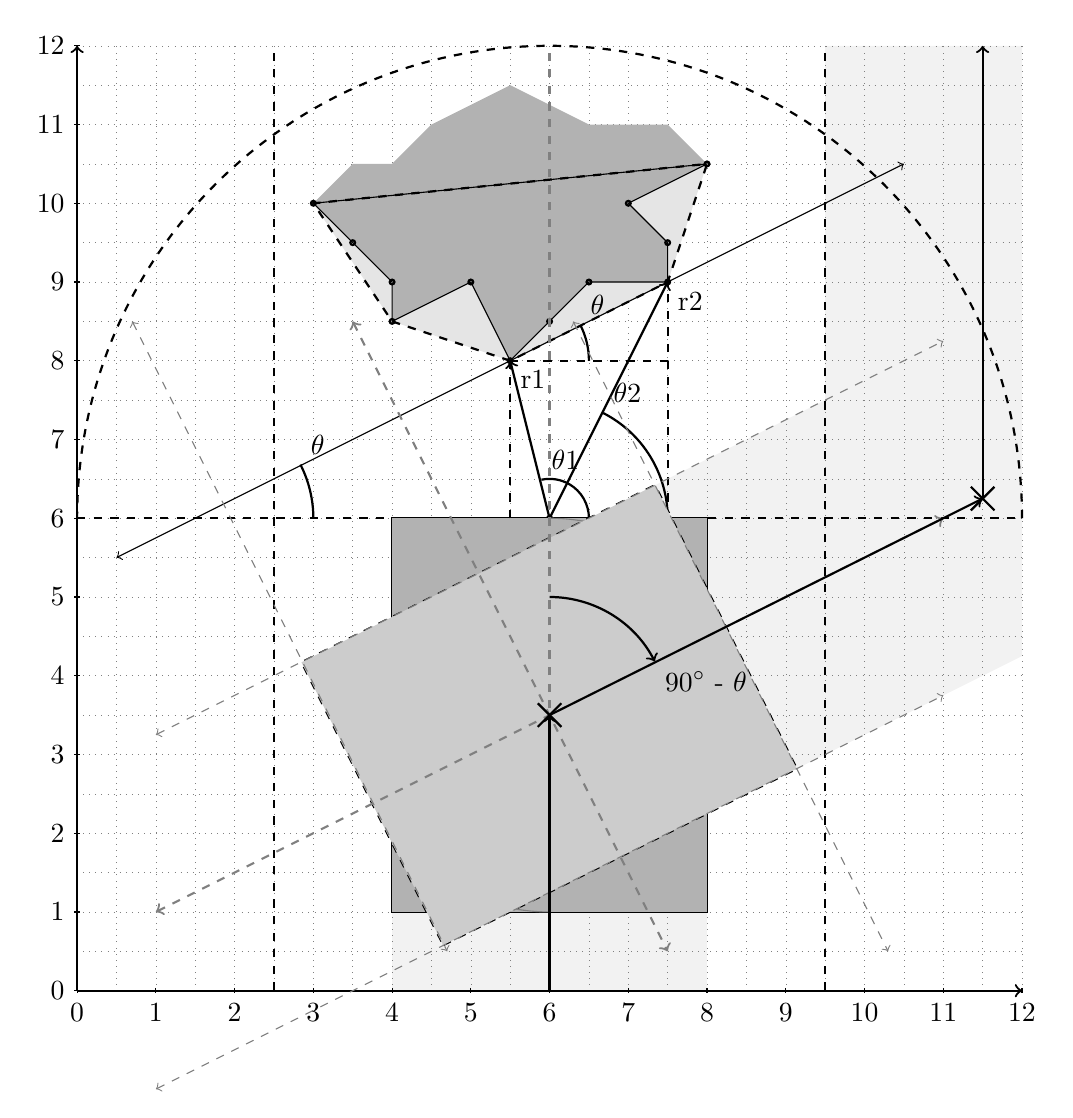
\begin{tikzpicture}
	\fill[black!5!white] (9.14, 2.82) -- (12, 4.25) -- (12, 12) -- (9.5, 12) -- (9.5, 7.5) -- (7.34, 6.42) -- cycle;
	\fill[black!5!white] (4, 0) -- (8, 0) -- (8, 1) -- (4, 1) -- cycle;
	
	\draw[step = 0.5 cm, gray, very thin, dotted] (0, 0) grid (12, 12);
	\draw[thick, ->] (0, 0) -- (12, 0);
	\draw[thick, ->] (0, 0) -- (0, 12);
	\foreach \x in {0, ..., 12}
		\draw (\x cm, 1 pt) -- (\x cm, -1 pt) node[anchor = north] {$\x$};
	\foreach \y in {0, ..., 12}
		\draw (1 pt, \y cm) -- (-1 pt, \y cm) node[anchor = east] {$\y$};	
	
	\fill[black!10!white] (4, 8.5) -- (5.5, 8) -- (7.5, 9) -- (8, 10.5) -- (3, 10) -- cycle;
	
	\fill[black!30!white] (4, 8.5) -- (5, 9) -- (5.5, 8) -- (6, 8.5) -- (6.5, 9) -- (7.5, 9) -- (7.5, 9.5) -- (7, 10) -- (8, 10.5) -- (7.5, 11) -- (6.5, 11) -- (5.5, 11.5) -- (4.5, 11) -- (4, 10.5) -- (3.5, 10.5) -- (3, 10) -- (3.5, 9.5) -- (4, 9) -- cycle;
	
	\draw[thick, dashed] (4, 8.5) -- (5.5, 8) -- (7.5, 9) -- (8, 10.5) -- (3, 10) -- cycle;
	
	\draw[thick] (4, 8.5) circle (0.03 cm);
	\draw[thick] (5.5, 8) circle (0.03 cm);
	\draw[thick] (7.5, 9) circle (0.03 cm);
	\draw[thick] (8, 10.5) circle (0.03 cm);
	\draw[thick] (3, 10) circle (0.03 cm);
	\draw[thick] (3.5, 9.5) circle (0.03 cm);
	\draw[thick] (4, 9) circle (0.03 cm);
	\draw[thick] (5, 9) circle (0.03 cm);
	\draw[thick] (6, 8.5) circle (0.03 cm);
	\draw[thick] (6.5, 9) circle (0.03 cm);
	\draw[thick] (7.5, 9.5) circle (0.03 cm);
	\draw[thick] (7, 10) circle (0.03 cm);
	
	\draw[thin] (4, 8.5) -- (5, 9) -- (5.5, 8) -- (6, 8.5) -- (6.5, 9) -- (7.5, 9) -- (7.5, 9.5) -- (7, 10) -- (8, 10.5) -- (3, 10) -- (3.5, 9.5) -- (4, 9) -- cycle;
	
	\draw[<->] (0.5, 5.5) -- (10.5, 10.5);
	\draw[thick] (3, 6) arc (0:27:1.5) node[anchor = south west] {$\theta$};
	
	\draw[thick, dashed] (12, 6) arc (0: 180: 6); 
	\draw[thick, dashed] (2.5, 0) -- (2.5, 12);
	\draw[thick, dashed] (9.5, 0) -- (9.5, 12);
	\draw[thick, dashed] (0, 6) -- (12, 6);
	
	\draw[thick] (4, 1) -- (8, 1) -- (8, 6) -- (4, 6) -- cycle;
	\draw[thick] (6, 6) circle (0.03 cm);
	\fill[black!30!white] (4, 1) rectangle (8, 6);
	
	\draw[thick, ->] (6, 6) -- (5.5, 8) node[anchor = north west] {r1};
	\draw[thick] (6.5, 6) arc (0:102:0.5) node[anchor = south west] {$\theta$1};
	
	\draw[thick, ->] (6, 6) -- (7.5, 9) node[anchor = north west] {r2};
	\draw[thick] (7.5, 6) arc (0:63:1.5) node[anchor = south west] {$\theta$2};
	
	\draw[thick, dashed] (5.5, 8) -- (7.5, 8);
	\draw[thick, dashed] (5.5, 6) -- (5.5, 8);
	\draw[thick, dashed] (7.5, 6) -- (7.5, 9);
	\draw[thick] (6.5, 8) arc (0:27:1) node[anchor = south west] {$\theta$};
	
	\draw[gray, thin] (4, 3.5) arc (180:90:2);
	\draw[gray, thin] (8, 3.5) arc (0:-90:2);
	\draw[gray, thin] (8.5, 3.5) arc (0:90:2.5);
	\draw[gray, thin] (6, 1) arc (270:180:2.5);
	
	\draw[thick, dashed] (4.65, 0.58) -- (9.14, 2.82) -- (7.34, 6.42) -- (2.85, 4.17) -- cycle;
	\fill[black!20!white] (4.65, 0.58) -- (9.14, 2.82) -- (7.34, 6.42) -- (2.85, 4.17) -- cycle;
	
	\draw[gray, thick, dashed, <->] (1, 1) -- (11, 6);
	\draw[gray, thick, dashed, <->] (3.5, 8.5) -- (7.5, 0.5);
	
	\draw[gray, thin, dashed, <->] (6.3, 8.5) -- (10.3, 0.5);
	\draw[gray, thin, dashed, <->] (0.7, 8.5) -- (4.7, 0.5);
	\draw[gray, thin, dashed, <->] (1, 3.25) -- (11, 8.25);
	\draw[gray, thin, dashed, <->] (1, -1.25) -- (11, 3.75);
	
	\draw[gray, thick, dashed] (6, 0) -- (6, 12);
	
	\draw[thick] (5.85, 3.35) -- (6.15, 3.65);
	\draw[thick] (5.85, 3.65) -- (6.15, 3.35);
	
	\draw[thick, ->] (6, 5) arc (90:27:1.5) node [anchor =  north west] {$90^{\circ}$ - $\theta$};
	
	\draw[thick] (11.35, 6.1) -- (11.65, 6.4);
	\draw[thick] (11.35, 6.4) -- (11.65, 6.1);
	
	\draw[thick, ->] (6, 3.5) -- (11.5, 6.25);
	\draw[thick, ->] (6, 0) -- (6, 3.5);
	\draw[thick, ->] (11.5, 6.25) -- (11.5, 12);
	\end{tikzpicture}
	
	\begin{align}
	\tan{\theta} & = \frac{h_{2} - h_{1}}{w_{2} - w_{1}} \\
	&= \frac{r_{2} \cos{\theta_{2}} - r_{1} \cos{\theta_{1}}}{r_{2} \sin{\theta_{2}} - r_{1} \sin{\theta_{1}}} \\
	\theta & = \arctan{\frac{r_{2} \cos{\theta_{2}} - r_{1} \cos{\theta_{1}}}{r_{2} \sin{\theta_{2}} - r_{1} \sin{\theta_{1}}}} \\
	\alpha & = 90^{\circ} - \theta \\
	& = \arctan{\frac{r_{2} \sin{\theta_{2}} - r_{1} \sin{\theta_{1}}}{r_{2} \cos{\theta_{2}} - r_{1} \cos{\theta_{1}}}}
	\end{align}
	
	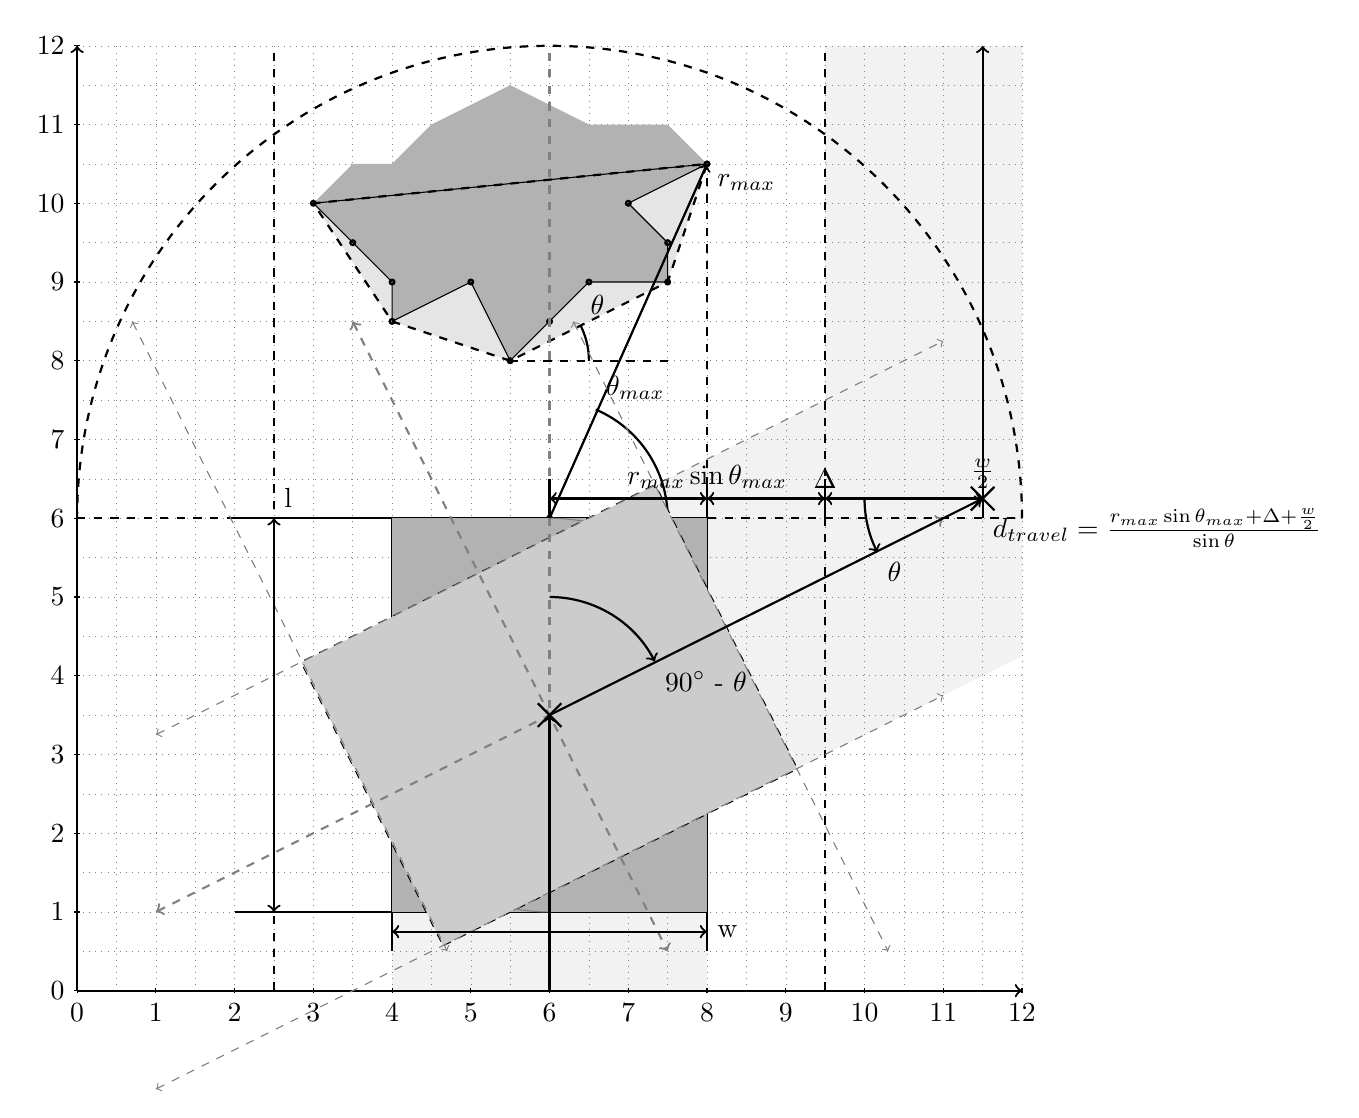
\begin{tikzpicture}
	\fill[black!5!white] (9.14, 2.82) -- (12, 4.25) -- (12, 12) -- (9.5, 12) -- (9.5, 7.5) -- (7.34, 6.42) -- cycle;
	\fill[black!5!white] (4, 0) -- (8, 0) -- (8, 1) -- (4, 1) -- cycle;
	
	\draw[step = 0.5 cm, gray, very thin, dotted] (0, 0) grid (12, 12);
	\draw[thick, ->] (0, 0) -- (12, 0);
	\draw[thick, ->] (0, 0) -- (0, 12);
	\foreach \x in {0, ..., 12}
	\draw (\x cm, 1 pt) -- (\x cm, -1 pt) node[anchor = north] {$\x$};
	\foreach \y in {0, ..., 12}
	\draw (1 pt, \y cm) -- (-1 pt, \y cm) node[anchor = east] {$\y$};	
	
	\fill[black!10!white] (4, 8.5) -- (5.5, 8) -- (7.5, 9) -- (8, 10.5) -- (3, 10) -- cycle;
	
	\fill[black!30!white] (4, 8.5) -- (5, 9) -- (5.5, 8) -- (6, 8.5) -- (6.5, 9) -- (7.5, 9) -- (7.5, 9.5) -- (7, 10) -- (8, 10.5) -- (7.5, 11) -- (6.5, 11) -- (5.5, 11.5) -- (4.5, 11) -- (4, 10.5) -- (3.5, 10.5) -- (3, 10) -- (3.5, 9.5) -- (4, 9) -- cycle;
	
	\draw[thick, dashed] (4, 8.5) -- (5.5, 8) -- (7.5, 9) -- (8, 10.5) -- (3, 10) -- cycle;
	
	\draw[thick] (4, 8.5) circle (0.03 cm);
	\draw[thick] (5.5, 8) circle (0.03 cm);
	\draw[thick] (7.5, 9) circle (0.03 cm);
	\draw[thick] (8, 10.5) circle (0.03 cm);
	\draw[thick] (3, 10) circle (0.03 cm);
	\draw[thick] (3.5, 9.5) circle (0.03 cm);
	\draw[thick] (4, 9) circle (0.03 cm);
	\draw[thick] (5, 9) circle (0.03 cm);
	\draw[thick] (6, 8.5) circle (0.03 cm);
	\draw[thick] (6.5, 9) circle (0.03 cm);
	\draw[thick] (7.5, 9.5) circle (0.03 cm);
	\draw[thick] (7, 10) circle (0.03 cm);
	
	\draw[thin] (4, 8.5) -- (5, 9) -- (5.5, 8) -- (6, 8.5) -- (6.5, 9) -- (7.5, 9) -- (7.5, 9.5) -- (7, 10) -- (8, 10.5) -- (3, 10) -- (3.5, 9.5) -- (4, 9) -- cycle;
	
	\draw[thick, dashed] (12, 6) arc (0: 180: 6); 
	\draw[thick, dashed] (2.5, 0) -- (2.5, 12);
	\draw[thick, dashed] (9.5, 0) -- (9.5, 12);
	\draw[thick, dashed] (0, 6) -- (12, 6);
	
	\draw[thick] (4, 1) -- (8, 1) -- (8, 6) -- (4, 6) -- cycle;
	\draw[thick] (6, 6) circle (0.03 cm);
	\fill[black!30!white] (4, 1) rectangle (8, 6);
	
	\draw[thick, ->] (6, 6) -- (8, 10.5) node[anchor = north west] {$r_{max}$};
	\draw[thick] (7.5, 6) arc (0:67:1.5) node[anchor = south west] {$\theta_{max}$};
	
	\draw[thick, dashed] (5.5, 8) -- (7.5, 8);
	\draw[thick, dashed] (8, 6) -- (8, 10.5);
	\draw[thick] (6.5, 8) arc (0:27:1) node[anchor = south west] {$\theta$};
	
	\draw[gray, thin] (4, 3.5) arc (180:90:2);
	\draw[gray, thin] (8, 3.5) arc (0:-90:2);
	\draw[gray, thin] (8.5, 3.5) arc (0:90:2.5);
	\draw[gray, thin] (6, 1) arc (270:180:2.5);
	
	\draw[thick, dashed] (4.65, 0.58) -- (9.14, 2.82) -- (7.34, 6.42) -- (2.85, 4.17) -- cycle;
	\fill[black!20!white] (4.65, 0.58) -- (9.14, 2.82) -- (7.34, 6.42) -- (2.85, 4.17) -- cycle;
	
	\draw[gray, thick, dashed, <->] (1, 1) -- (11, 6);
	\draw[gray, thick, dashed, <->] (3.5, 8.5) -- (7.5, 0.5);
	
	\draw[gray, thin, dashed, <->] (6.3, 8.5) -- (10.3, 0.5);
	\draw[gray, thin, dashed, <->] (0.7, 8.5) -- (4.7, 0.5);
	\draw[gray, thin, dashed, <->] (1, 3.25) -- (11, 8.25);
	\draw[gray, thin, dashed, <->] (1, -1.25) -- (11, 3.75);
	
	\draw[gray, thick, dashed] (6, 0) -- (6, 12);
	
	\draw[thick] (5.85, 3.35) -- (6.15, 3.65);
	\draw[thick] (5.85, 3.65) -- (6.15, 3.35);
	
	\draw[thick, ->] (6, 5) arc (90:27:1.5) node [anchor =  north west] {$90^{\circ}$ - $\theta$};
	
	\draw[thick] (11.35, 6.1) -- (11.65, 6.4);
	\draw[thick] (11.35, 6.4) -- (11.65, 6.1);
	
	\draw[thick, ->] (6, 3.5) -- (11.5, 6.25) node[anchor= north west] {$d_{travel} = \frac{r_{max}\sin{\theta_{max}} + \Delta + \frac{w}{2}}{\sin{\theta}}$};
	
	\draw[thick, ->] (6, 0) -- (6, 3.5);
	\draw[thick, ->] (11.5, 6.25) -- (11.5, 12);
	
	\draw[thick] (6, 6) -- (6, 6.5);
	\draw[thick, <->] (6, 6.25) -- (8, 6.25) node[anchor = south] {$r_{max}\sin{\theta_{max}}$};	
	\draw[thick] (8, 6) -- (8, 6.5);
	\draw[thick] (9.5, 6) -- (9.5, 6.5);
	\draw[thick, <->] (8, 6.25) -- (9.5, 6.25) node[anchor = south] {$\Delta$};
	
	\draw[thick] (11.5, 6) -- (11.5, 6.5);
	\draw[thick, <->] (9.5, 6.25) -- (11.5, 6.25) node[anchor = south] {$\frac{w}{2}$};
	
	\draw[thick, ->] (10, 6.25) arc (180:207:1.5) node [anchor =  north west] {$\theta$};
	
	\draw[thick] (2, 1) -- (4, 1);
	\draw[thick] (2, 6) -- (4, 6);
	\draw[thick, <->] (2.5, 1) -- (2.5, 6) node[anchor = south west] {l};
	
	\draw[thick] (4, 0.5) -- (4, 1);
	\draw[thick] (8, 0.5) -- (8, 1);
	\draw[thick, <->] (4, 0.75) -- (8, 0.75) node[anchor = west] {w};
	\end{tikzpicture}
	
	\begin{align}
	d_{travel} \sin{\theta} &= r_{max}\sin{\theta_{max}} + \Delta + \frac{w}{2} \\
	d_{travel} &= \frac{r_{max}\sin{\theta_{max}} + \Delta + \frac{w}{2}}{\sin{\theta}}
	\end{align}
	
	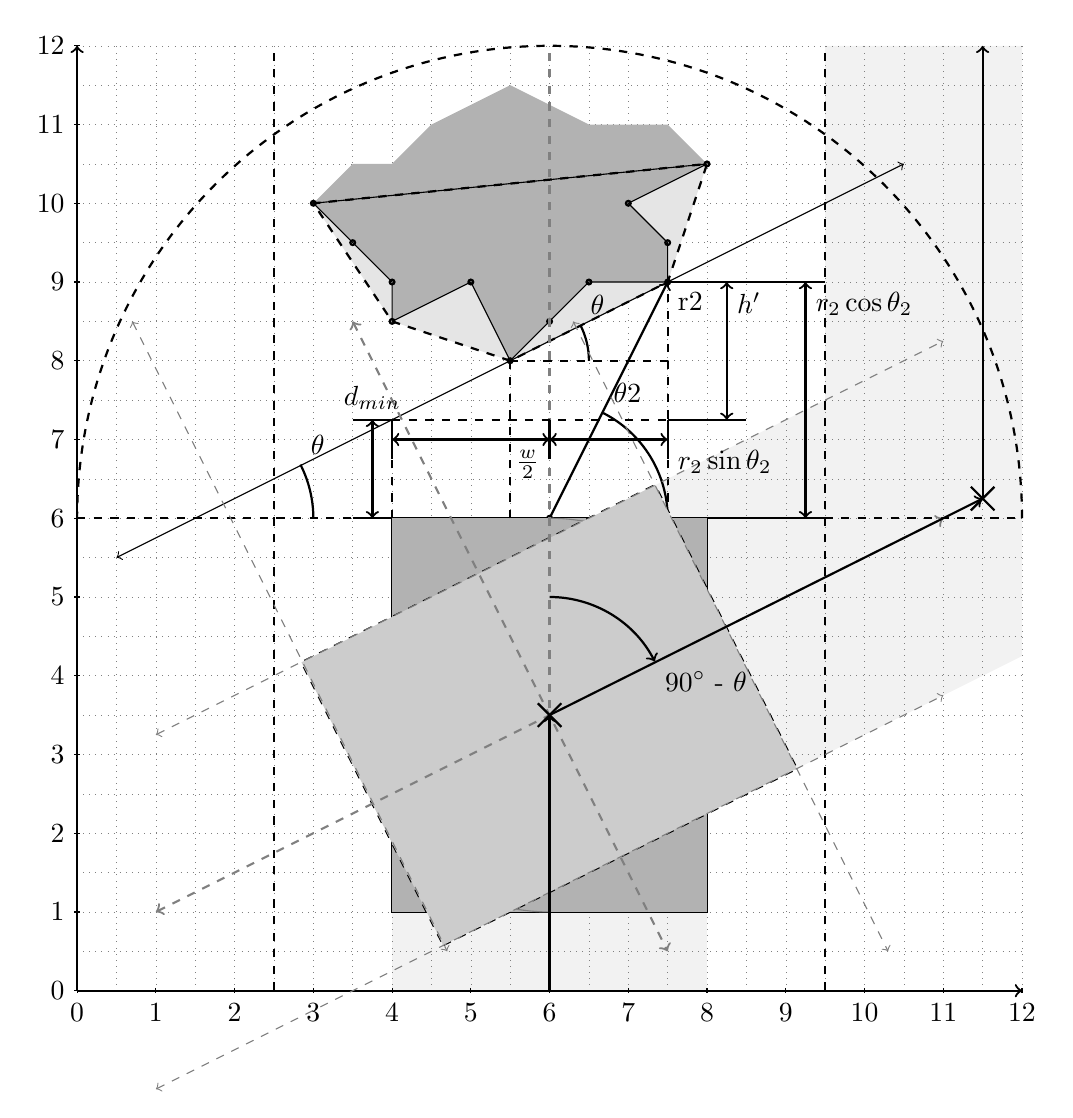
\begin{tikzpicture}
	\fill[black!5!white] (9.14, 2.82) -- (12, 4.25) -- (12, 12) -- (9.5, 12) -- (9.5, 7.5) -- (7.34, 6.42) -- cycle;
	\fill[black!5!white] (4, 0) -- (8, 0) -- (8, 1) -- (4, 1) -- cycle;
	
	\draw[step = 0.5 cm, gray, very thin, dotted] (0, 0) grid (12, 12);
	\draw[thick, ->] (0, 0) -- (12, 0);
	\draw[thick, ->] (0, 0) -- (0, 12);
	\foreach \x in {0, ..., 12}
	\draw (\x cm, 1 pt) -- (\x cm, -1 pt) node[anchor = north] {$\x$};
	\foreach \y in {0, ..., 12}
	\draw (1 pt, \y cm) -- (-1 pt, \y cm) node[anchor = east] {$\y$};	
	
	\fill[black!10!white] (4, 8.5) -- (5.5, 8) -- (7.5, 9) -- (8, 10.5) -- (3, 10) -- cycle;
	
	\fill[black!30!white] (4, 8.5) -- (5, 9) -- (5.5, 8) -- (6, 8.5) -- (6.5, 9) -- (7.5, 9) -- (7.5, 9.5) -- (7, 10) -- (8, 10.5) -- (7.5, 11) -- (6.5, 11) -- (5.5, 11.5) -- (4.5, 11) -- (4, 10.5) -- (3.5, 10.5) -- (3, 10) -- (3.5, 9.5) -- (4, 9) -- cycle;
	
	\draw[thick, dashed] (4, 8.5) -- (5.5, 8) -- (7.5, 9) -- (8, 10.5) -- (3, 10) -- cycle;
	
	\draw[thick] (4, 8.5) circle (0.03 cm);
	\draw[thick] (5.5, 8) circle (0.03 cm);
	\draw[thick] (7.5, 9) circle (0.03 cm);
	\draw[thick] (8, 10.5) circle (0.03 cm);
	\draw[thick] (3, 10) circle (0.03 cm);
	\draw[thick] (3.5, 9.5) circle (0.03 cm);
	\draw[thick] (4, 9) circle (0.03 cm);
	\draw[thick] (5, 9) circle (0.03 cm);
	\draw[thick] (6, 8.5) circle (0.03 cm);
	\draw[thick] (6.5, 9) circle (0.03 cm);
	\draw[thick] (7.5, 9.5) circle (0.03 cm);
	\draw[thick] (7, 10) circle (0.03 cm);
	
	\draw[thin] (4, 8.5) -- (5, 9) -- (5.5, 8) -- (6, 8.5) -- (6.5, 9) -- (7.5, 9) -- (7.5, 9.5) -- (7, 10) -- (8, 10.5) -- (3, 10) -- (3.5, 9.5) -- (4, 9) -- cycle;
	
	\draw[<->] (0.5, 5.5) -- (10.5, 10.5);
	\draw[thick] (3, 6) arc (0:27:1.5) node[anchor = south west] {$\theta$};
	
	\draw[thick, dashed] (12, 6) arc (0: 180: 6); 
	\draw[thick, dashed] (2.5, 0) -- (2.5, 12);
	\draw[thick, dashed] (9.5, 0) -- (9.5, 12);
	\draw[thick, dashed] (0, 6) -- (12, 6);
	
	\draw[thick] (4, 1) -- (8, 1) -- (8, 6) -- (4, 6) -- cycle;
	\draw[thick] (6, 6) circle (0.03 cm);
	\fill[black!30!white] (4, 1) rectangle (8, 6);
	
	\draw[thick, ->] (6, 6) -- (7.5, 9) node[anchor = north west] {r2};
	\draw[thick] (7.5, 6) arc (0:63:1.5) node[anchor = south west] {$\theta$2};
	
	\draw[thick, dashed] (5.5, 8) -- (7.5, 8);
	\draw[thick, dashed] (5.5, 6) -- (5.5, 8);
	\draw[thick, dashed] (7.5, 6) -- (7.5, 9);
	\draw[thick] (6.5, 8) arc (0:27:1) node[anchor = south west] {$\theta$};
	
	\draw[gray, thin] (4, 3.5) arc (180:90:2);
	\draw[gray, thin] (8, 3.5) arc (0:-90:2);
	\draw[gray, thin] (8.5, 3.5) arc (0:90:2.5);
	\draw[gray, thin] (6, 1) arc (270:180:2.5);
	
	\draw[thick, dashed] (4.65, 0.58) -- (9.14, 2.82) -- (7.34, 6.42) -- (2.85, 4.17) -- cycle;
	\fill[black!20!white] (4.65, 0.58) -- (9.14, 2.82) -- (7.34, 6.42) -- (2.85, 4.17) -- cycle;
	
	\draw[gray, thick, dashed, <->] (1, 1) -- (11, 6);
	\draw[gray, thick, dashed, <->] (3.5, 8.5) -- (7.5, 0.5);
	
	\draw[gray, thin, dashed, <->] (6.3, 8.5) -- (10.3, 0.5);
	\draw[gray, thin, dashed, <->] (0.7, 8.5) -- (4.7, 0.5);
	\draw[gray, thin, dashed, <->] (1, 3.25) -- (11, 8.25);
	\draw[gray, thin, dashed, <->] (1, -1.25) -- (11, 3.75);
	
	\draw[gray, thick, dashed] (6, 0) -- (6, 12);
	
	\draw[thick] (5.85, 3.35) -- (6.15, 3.65);
	\draw[thick] (5.85, 3.65) -- (6.15, 3.35);
	
	\draw[thick, ->] (6, 5) arc (90:27:1.5) node [anchor =  north west] {$90^{\circ}$ - $\theta$};
	
	\draw[thick] (11.35, 6.1) -- (11.65, 6.4);
	\draw[thick] (11.35, 6.4) -- (11.65, 6.1);
	
	\draw[thick, ->] (6, 3.5) -- (11.5, 6.25);
	\draw[thick, ->] (6, 0) -- (6, 3.5);
	\draw[thick, ->] (11.5, 6.25) -- (11.5, 12);
	
	\draw[thick, dashed] (4, 6) -- (4, 7.25);
	\draw[thick] (3.5, 6) -- (4, 6);
	\draw[thick] (3.5, 7.25) -- (4, 7.25);
	\draw[thick, <->] (3.75, 6) -- (3.75, 7.25) node[anchor = south] {$d_{min}$};
	
	\draw[thick, dashed] (4, 7.25) -- (7.5, 7.25);
	\draw[thick] (4, 6.75) -- (4, 7.25);
	\draw[thick] (6, 6.75) -- (6, 7.25);
	\draw[thick, <->] (4, 7) -- (6, 7) node[anchor = north east] {$\frac{w}{2}$};
	
	\draw[thick] (7.5, 6.75) -- (7.5, 7.25);
	\draw[thick, <->] (6, 7) -- (7.5, 7) node[anchor = north west] {$r_{2} \sin{\theta_{2}}$};
	
	\draw[thick] (7.5, 7.25) -- (8.5, 7.25);
	\draw[thick] (7.5, 9) -- (9.5, 9);
	\draw[thick, <->] (8.25, 7.25) -- (8.25, 9) node[anchor = north west] {$h^{\prime}$};
	\draw[thick] (8, 6) -- (9.5, 6);
	\draw[thick, <->] (9.25, 6) -- (9.25, 9) node[anchor = north west] {$r_{2} \cos{\theta_{2}}$};
	\end{tikzpicture}
	
	\begin{align}
	h^{\prime} &= \left(\frac{w}{2} + r_{2} \sin{\theta_{2}}\right) \tan{\theta} \\
	d_{min} &= r_{2} \cos{\theta_{2}} - h^{\prime} \\
	&= r_{2} \cos{\theta_{2}} - \left(\frac{w}{2} + r_{2} \sin{\theta_{2}}\right) \tan{\theta} \\
	&= r_{2} \cos{\theta_{2}} - \left(\frac{w}{2}\right) \tan{\theta} - r_{2} \sin{\theta_{2}} \tan{\theta} \\
	&= r_{2} \cos{\theta_{2}} - r_{2} \sin{\theta_{2}} \left(\frac{\sin{\theta}}{\cos{\theta}}\right) - \left(\frac{w}{2}\right) \tan{\theta} \\
	&= \frac{r_{2}}{\cos{\theta}} \left(\cos{\theta_{2}} \cos{\theta} - \sin{\theta_{2}} \sin{\theta}\right) - \left(\frac{w}{2}\right) \tan{\theta} \\
	&= \left(\frac{r_{2}}{\cos{\theta}}\right) \cos{\left(\theta_{2} + \theta\right)} - \left(\frac{w}{2}\right) \tan{\theta} \\
	d_{min} &= \left(r_{2} \cos{\left(\theta_{2} + \theta\right)} - \left(\frac{w}{2}\right) \sin{\theta}\right) \frac{1}{\cos{\theta}}
	\end{align}
	
	\begin{align}
	d_{min} &\ge \Delta_{min}
	\end{align}
	
	\begin{align}
	t_{hit} &= \frac{d_{min}}{v_{robo}} \\
	\implies t_{decision} &\le t_{hit}
	\end{align}
	
	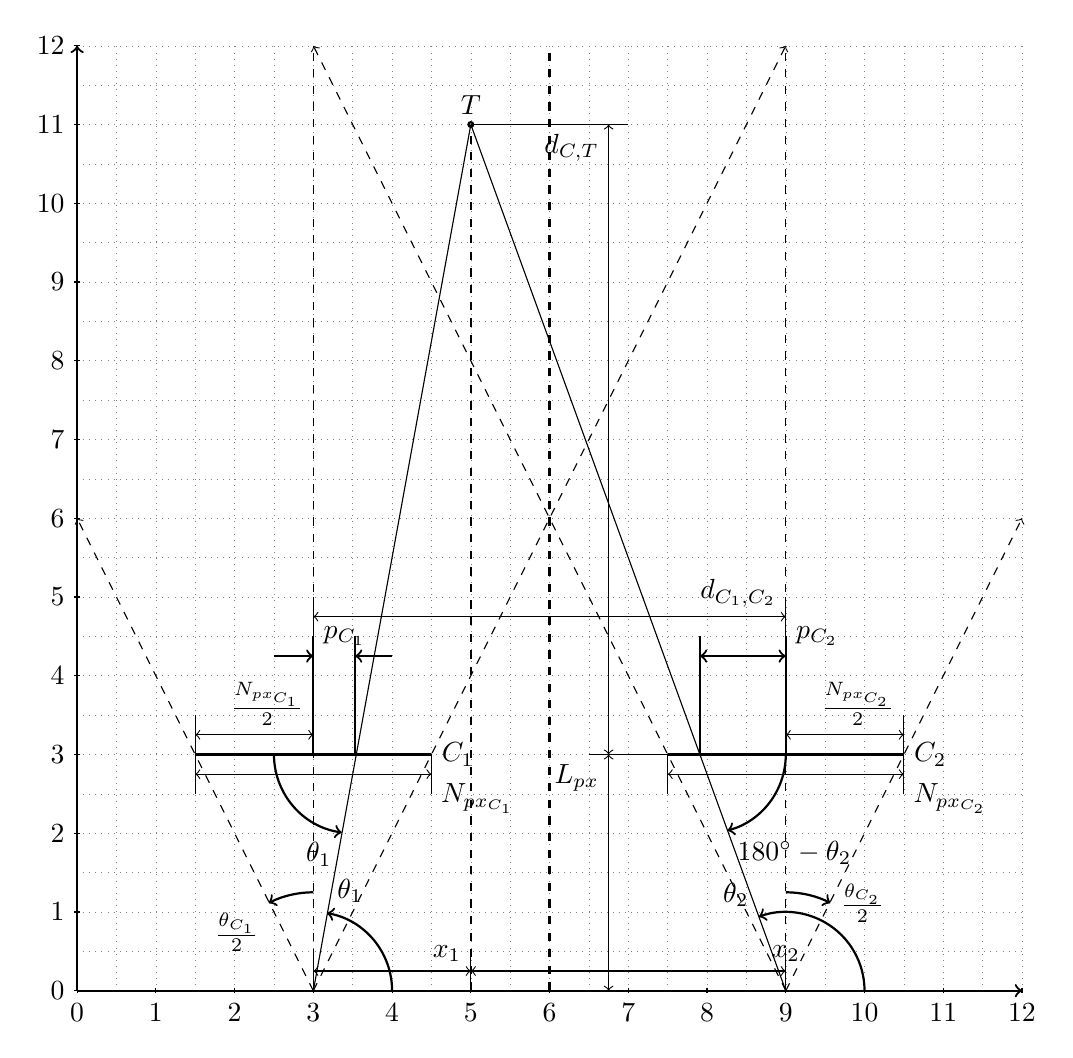
\begin{tikzpicture}
		\draw[step = 0.5 cm, gray, very thin, dotted] (0, 0) grid (12, 12);
		\draw[thick, ->] (0, 0) -- (12, 0);
		\draw[thick, ->] (0, 0) -- (0, 12);
		\foreach \x in {0, ..., 12}
		\draw (\x cm, 1 pt) -- (\x cm, -1 pt) node[anchor = north] {$\x$};
		\foreach \y in {0, ..., 12}
		\draw (1 pt, \y cm) -- (-1 pt, \y cm) node[anchor = east] {$\y$};	
		
		\draw[thick, dashed] (6, 0) -- (6, 12);
		
		\draw[thin, dashed, ->] (3, 0) -- (0, 6);
		\draw[thin, dashed, ->] (3, 0) -- (9, 12);
		\draw[thin, dashed] (3, 0) -- (3, 12);
		
		\draw[thin, dashed, ->] (9, 0) -- (3, 12);
		\draw[thin, dashed, ->] (9, 0) -- (12, 6);
		\draw[thin, dashed] (9, 0) -- (9, 12);
		
		\draw[thick] (5, 11) circle (0.03 cm) node[anchor = south] {$T$};
		
		\draw[thick] (1.5, 3) -- (4.5, 3) node [anchor = west] {$C_{1}$};
		
		\draw[thick] (7.5, 3) -- (10.5, 3) node [anchor = west] {$C_{2}$};;
		
		\draw[thin] (3, 0) -- (5, 11);
		\draw[thin] (5, 11) -- (9, 0);
		
		\draw[thick, dashed] (5, 0) -- (5, 11);
		
		\draw [thick] (3, 3) -- (3, 4.5);
		\draw [thick] (3.53, 3) -- (3.53, 4.5);
		\draw [thick, ->] (2.5, 4.25) -- (3, 4.25) node[anchor = south west] {$p_{C_{1}}$};
		\draw [thick, ->] (4, 4.25) -- (3.53, 4.25);
		
		\draw [thick] (7.91, 3) -- (7.91, 4.5);
		\draw [thick] (9, 3) -- (9, 4.5);
		\draw [thick, <->] (7.91, 4.25) -- (9, 4.25) node[anchor = south west] {$p_{C_{2}}$};
		
		\draw[thick, ->] (4, 0) arc (0:80:1) node[anchor = south west] {$\theta_{1}$}; 
		
		\draw[thick, ->] (10, 0) arc (0:110:1) node[anchor = south east] {$\theta_{2}$}; 
		
		\draw[thin] (1.5, 2.5) -- (1.5, 3);
		\draw[thin] (4.5, 2.5) -- (4.5, 3);
		\draw[thin, <->] (1.5, 2.75) -- (4.5, 2.75) node[anchor = north west] {$N_{px_{C_{1}}}$};
		
		\draw[thin] (7.5, 2.5) -- (7.5, 3);
		\draw[thin] (10.5, 2.5) -- (10.5, 3);
		\draw[thin, <->] (7.5, 2.75) -- (10.5, 2.75) node[anchor = north west] {$N_{px_{C_{2}}}$};
		
		\draw[thin] (6.5, 3) -- (7.5, 3);
		\draw[thin, <->] (6.75, 0) -- (6.75, 3) node[anchor = north east] {$L_{px}$};
		
		\draw[thin] (5, 11) -- (7, 11);
		\draw[thin, <->] (6.75, 3) -- (6.75, 11) node[anchor = north east] {$d_{C, T}$};
		
		\draw[thick, ->] (2.5, 3) arc (180:262:1) node[anchor = north east] {$\theta_{1}$};
		
		\draw[thick, ->] (9, 3) arc (0:-75:1) node[anchor = north west] {$180^{\circ} - \theta_{2}$};
		
		\draw[thick, ->] (3, 1.25) arc (90:117:1.25) node[anchor = north east] {$\frac{\theta_{C_{1}}}{2}$}; 
		
		\draw[thick, ->] (9, 1.25) arc (90:63:1.25) node[anchor = west] {$\frac{\theta_{C_{2}}}{2}$}; 
		
		\draw[thin] (10.5, 3) -- (10.5, 3.5);
		\draw[thin, <->] (9, 3.25) -- (10.5, 3.25) node[anchor = south east] {$\frac{N_{px_{C_{2}}}}{2}$};
		
		\draw[thin] (1.5, 3) -- (1.5, 3.5);
		\draw[thin, <->] (1.5, 3.25) -- (3, 3.25) node[anchor = south east] {$\frac{N_{px_{C_{1}}}}{2}$};
		
		\draw[thin] (3, 0) -- (3, 0.5);
		\draw[thin] (5, 0) -- (5, 0.5);
		\draw[thin, <->] (3, 0.25) -- (5, 0.25) node[anchor = south east] {$x_{1}$}; 
		
		\draw[thin] (9, 0) -- (9, 0.5);
		\draw[thin, <->] (5, 0.25) -- (9, 0.25) node[anchor = south] {$x_{2}$}; 
		
		\draw[thin] (3, 4.5) -- (3, 5);
		\draw[thin] (9, 4.5) -- (9, 5);
		\draw[thin, <->] (3, 4.75) -- (9, 4.75) node[anchor = south east] {$d_{C_{1}, C_{2}}$}; 
	\end{tikzpicture}
	
	\begin{align}
	\tan \left(\frac{\theta_{C_{1}}}{2}\right) &=  \frac{\left(\frac{N_{px_{C_{1}}}}{2}\right)}{L_{px}} \\
	\implies L_{px} &= \left(\frac{N_{px_{C_{1}}}}{2}\right) \frac{1}{\tan \left(\frac{\theta_{C_{1}}}{2}\right)} \\
	&= \frac{N_{px_{C_{1}}}}{2 \tan \left(\frac{\theta_{C_{1}}}{2}\right)} \\
	\tan \theta_{1} &= \frac{L_{px}}{p_{C_{1}}} \\
	&= \frac{\left(\frac{N_{px_{C_{1}}}}{2 \tan \left(\frac{\theta_{C_{1}}}{2}\right)}\right)}{p_{C_{1}}} \\
	&= \frac{N_{px_{C_{1}}}}{2 p_{C_{1}} \tan \left(\frac{\theta_{C_{1}}}{2}\right)} \\
	\implies \frac{1}{\tan \theta_{1}} &= \frac{2 p_{C_{1}} \tan \left(\frac{\theta_{C_{1}}}{2}\right)}{N_{px_{C_{1}}}} \\
	\tan \left(180^{\circ} - \theta_{2}\right) &= \frac{L_{px}}{p_{C_{2}}} \\
	&= \frac{\left(\frac{N_{px_{C_{2}}}}{2 \tan \left(\frac{\theta_{C_{2}}}{2}\right)}\right)}{p_{C_{2}}} \\
	&= \frac{N_{px_{C_{2}}}}{2 p_{C_{2}} \tan \left(\frac{\theta_{C_{2}}}{2}\right)} \\
	\implies \tan \theta_{2} &= -\left(\frac{N_{px_{C_{2}}}}{2 p_{C_{2}} \tan \left(\frac{\theta_{C_{2}}}{2}\right)}\right) \\
	\implies \frac{1}{\tan \theta_{2}} &= -\left(\frac{2 p_{C_{2}} \tan \left(\frac{\theta_{C_{2}}}{2}\right)}{N_{px_{C_{2}}}}\right)
	\end{align}
	
	\begin{align}
	Let &: \sigma_{px/unit} be density of pixels per unit of measurement \\
	Let &: L_{units} = \frac{L_{px}}{\sigma_{px/unit}} \\
	\tan \theta_{1} &= \frac{d_{C, T} + L_{units}}{x_{1}} \\
	\tan \theta_{1} &= \frac{d_{C, T} + L_{units}}{x_{1}} \\
	\implies x_{1} &= \frac{d_{C, T} + L_{units}}{\tan \theta_{1}} \\
	\tan \left({180^{\circ} - \theta_{2}}\right) &= \frac{d_{C, T} + L_{units}}{x_{2}} \\
	\implies x_{2} &= \frac{d_{C, T} + L_{px}}{\tan \left({180^{\circ} - \theta_{2}}\right)} \\
	\implies x_{1} + x_{2} &= \frac{d_{C, T} + L_{units}}{\tan \theta_{1}} + \frac{d_{C, T} + L_{units}}{\tan \left({180^{\circ} - \theta_{2}}\right)} \\
	&= \left(d_{C, T} + L_{units}\right) \left(\frac{1}{\tan \theta_{1}} + \frac{1}{\tan \left({180^{\circ} - \theta_{2}}\right)}\right) \\
	&= \left(d_{C, T} + L_{units}\right) \left(\frac{1}{\tan \theta_{1}} - \frac{1}{\tan \theta_{2}}\right) \\
	&= \left(d_{C, T} + L_{units}\right) \left(\frac{\tan \theta_{2} - \tan \theta_{1}}{\tan \theta_{1} \tan \theta_{2}}\right) \\
	\end{align}
	
	\begin{align}
	x_{1} + x_{2} &= d_{C_{1}, C_{2}} \\
	\implies d_{C_{1}, C_{2}} &= \left(d_{C, T} + L_{units}\right) \left(\frac{\tan \theta_{2} - \tan \theta_{1}}{\tan \theta_{1} \tan \theta_{2}}\right) \\
	\implies d_{C, T} + L_{units} &= d_{C_{1}, C_{2}} \left(\frac{\tan \theta_{1} \tan \theta_{2}}{\tan \theta_{2} - \tan \theta_{1}}\right) \\
	&= \frac{d_{C_{1}, C_{2}} \tan \theta_{1} \tan \theta_{2}}{\tan \theta_{2} - \tan \theta_{1}} \\
	\implies d_{C, T} &= \frac{d_{C_{1}, C_{2}} \tan \theta_{1} \tan \theta_{2}}{\tan \theta_{2} - \tan \theta_{1}} - L_{units} \\
	\implies d_{C, T} &= \frac{d_{C_{1}, C_{2}} \tan \theta_{1} \tan \theta_{2}}{\tan \theta_{2} - \tan \theta_{1}} - \frac{N_{px_{C_{1}}}}{2 \tan \left(\frac{\theta_{C_{1}}}{2}\right) \sigma_{px / unit}} \\
	\implies d_{C, T} &= \frac{d_{C_{1}, C_{2}}}{\left(\frac{1}{\tan \theta_{1}} - \frac{1}{\tan \theta_{2}}\right)} - \frac{N_{px_{C_{1}}}}{2 \tan \left(\frac{\theta_{C_{1}}}{2}\right) \sigma_{px / unit}} \\
	&= \frac{d_{C_{1}, C_{2}}}{\left(\frac{1}{\tan \theta_{1}} - \frac{1}{\tan \theta_{2}}\right)} - \frac{N_{px_{C_{1}}}}{2 \tan \left(\frac{\theta_{C_{1}}}{2}\right) \sigma_{px / unit}} \\
	&= \frac{d_{C_{1}, C_{2}}}{\left(\frac{2 p_{C_{1}} \tan \left(\frac{\theta_{C_{1}}}{2}\right)}{N_{px_{C_{1}}}} + \frac{2 p_{C_{2}} \tan \left(\frac{\theta_{C_{2}}}{2}\right)}{N_{px_{C_{2}}}}\right)} - \frac{N_{px_{C_{1}}}}{2 \tan \left(\frac{\theta_{C_{1}}}{2}\right) \sigma_{px / unit}}
	\end{align}
	
	\begin{align}
		Let &: \tan \left(\frac{\theta_{C_{1}}}{2}\right) = \tan \left(\frac{\theta_{C_{2}}}{2}\right) = \tan \left(\frac{\theta_{C}}{2}\right) \\
		Let &: N_{px_{C_{1}}} = N_{px_{C_{2}}} = N_{px_{C}} \\
		\implies d_{C, T} &= \frac{d_{C_{1}, C_{2}}}{\left(\frac{2 p_{C_{1}} \tan \left(\frac{\theta_{C}}{2}\right)}{N_{px_{C}}} + \frac{2 p_{C_{2}} \tan \left(\frac{\theta_{C}}{2}\right)}{N_{px_{C}}}\right)} - \frac{N_{px_{C}}}{2 \tan \left(\frac{\theta_{C}}{2}\right) \sigma_{px / unit}} \\
		&= \frac{d_{C_{1}, C_{2}}}{\left(\frac{2 \tan \left(\frac{\theta_{C}}{2}\right)}{N_{px_{C}}}\right) \left(p_{C_{1}} + p_{C_{2}}\right)} - \frac{N_{px_{C}}}{2 \tan \left(\frac{\theta_{C}}{2}\right) \sigma_{px / unit}} \\
		&= \frac{d_{C_{1}, C_{2}} N_{px_{C}}}{2 \tan \left(\frac{\theta_{C}}{2}\right) \left(p_{C_{1}} + p_{C_{2}}\right)} - \frac{N_{px_{C}}}{2 \tan \left(\frac{\theta_{C}}{2}\right) \sigma_{px / unit}} \\
		&= \left(\frac{N_{px_{C}}}{2 \tan \left(\frac{\theta_{C}}{2}\right)}\right) \left(\frac{d_{C_{1}, C_{2}}}{p_{C_{1}} + p_{C_{2}}} - \frac{1}{\sigma_{px / unit}}\right) \\
		If &: \frac{1}{\sigma_{px/unit}} \ll \frac{d_{C_{1}, C_{2}}}{p_{C_{1}} + p_{C_{2}}} \\
		d_{C, T} &\approx \frac{N_{px_{C}} d_{C_{1}, C_{2}}}{2 \tan \left(\frac{\theta_{C}}{2}\right) \left(p_{C_{1}} + p_{C_{2}}\right)}
	\end{align}
	
	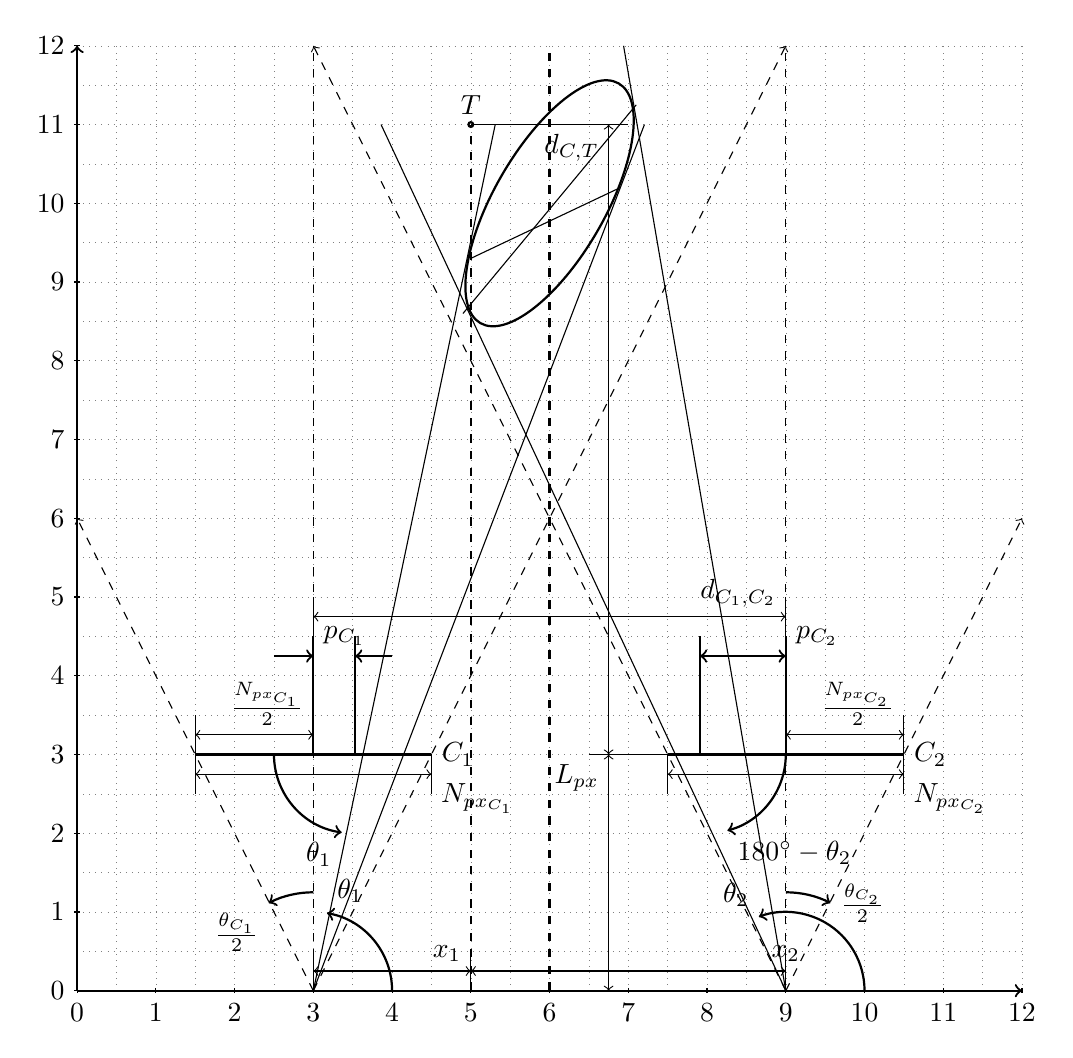
\begin{tikzpicture}
	\draw[step = 0.5 cm, gray, very thin, dotted] (0, 0) grid (12, 12);
	\draw[thick, ->] (0, 0) -- (12, 0);
	\draw[thick, ->] (0, 0) -- (0, 12);
	\foreach \x in {0, ..., 12}
	\draw (\x cm, 1 pt) -- (\x cm, -1 pt) node[anchor = north] {$\x$};
	\foreach \y in {0, ..., 12}
	\draw (1 pt, \y cm) -- (-1 pt, \y cm) node[anchor = east] {$\y$};	
	
	\draw[thick, dashed] (6, 0) -- (6, 12);
	
	\draw[thin, dashed, ->] (3, 0) -- (0, 6);
	\draw[thin, dashed, ->] (3, 0) -- (9, 12);
	\draw[thin, dashed] (3, 0) -- (3, 12);
	
	\draw[thin, dashed, ->] (9, 0) -- (3, 12);
	\draw[thin, dashed, ->] (9, 0) -- (12, 6);
	\draw[thin, dashed] (9, 0) -- (9, 12);
	
	\draw[thick] (5, 11) circle (0.03 cm) node[anchor = south] {$T$};
	
	\draw[thick] (1.5, 3) -- (4.5, 3) node [anchor = west] {$C_{1}$};
	
	\draw[thick] (7.5, 3) -- (10.5, 3) node [anchor = west] {$C_{2}$};;
	
	\draw[thin] (3, 0) -- (5.31, 11);
	\draw[thin] (3, 0) -- (7.205, 11);
	\draw[thin] (3.86, 11) -- (9, 0);
	\draw[thin] (6.94, 12) -- (9, 0);
	\draw[thin] (5, 9.3) -- (6.9, 10.2);
	\draw[thin] (4.9, 8.6) -- (7.1, 11.25);
	
	\draw[thick, dashed] (5, 0) -- (5, 11);
	
	\draw [thick] (3, 3) -- (3, 4.5);
	\draw [thick] (3.53, 3) -- (3.53, 4.5);
	\draw [thick, ->] (2.5, 4.25) -- (3, 4.25) node[anchor = south west] {$p_{C_{1}}$};
	\draw [thick, ->] (4, 4.25) -- (3.53, 4.25);
	
	\draw [thick] (7.91, 3) -- (7.91, 4.5);
	\draw [thick] (9, 3) -- (9, 4.5);
	\draw [thick, <->] (7.91, 4.25) -- (9, 4.25) node[anchor = south west] {$p_{C_{2}}$};
	
	\draw[thick, ->] (4, 0) arc (0:80:1) node[anchor = south west] {$\theta_{1}$}; 
	
	\draw[thick, ->] (10, 0) arc (0:110:1) node[anchor = south east] {$\theta_{2}$}; 
	
	\draw[thin] (1.5, 2.5) -- (1.5, 3);
	\draw[thin] (4.5, 2.5) -- (4.5, 3);
	\draw[thin, <->] (1.5, 2.75) -- (4.5, 2.75) node[anchor = north west] {$N_{px_{C_{1}}}$};
	
	\draw[thin] (7.5, 2.5) -- (7.5, 3);
	\draw[thin] (10.5, 2.5) -- (10.5, 3);
	\draw[thin, <->] (7.5, 2.75) -- (10.5, 2.75) node[anchor = north west] {$N_{px_{C_{2}}}$};
	
	\draw[thin] (6.5, 3) -- (7.5, 3);
	\draw[thin, <->] (6.75, 0) -- (6.75, 3) node[anchor = north east] {$L_{px}$};
	
	\draw[thin] (5, 11) -- (7, 11);
	\draw[thin, <->] (6.75, 3) -- (6.75, 11) node[anchor = north east] {$d_{C, T}$};
	
	\draw[thick, ->] (2.5, 3) arc (180:262:1) node[anchor = north east] {$\theta_{1}$};
	
	\draw[thick, ->] (9, 3) arc (0:-75:1) node[anchor = north west] {$180^{\circ} - \theta_{2}$};
	
	\draw[thick, ->] (3, 1.25) arc (90:117:1.25) node[anchor = north east] {$\frac{\theta_{C_{1}}}{2}$}; 
	
	\draw[thick, ->] (9, 1.25) arc (90:63:1.25) node[anchor = west] {$\frac{\theta_{C_{2}}}{2}$}; 
	
	\draw[thin] (10.5, 3) -- (10.5, 3.5);
	\draw[thin, <->] (9, 3.25) -- (10.5, 3.25) node[anchor = south east] {$\frac{N_{px_{C_{2}}}}{2}$};
	
	\draw[thin] (1.5, 3) -- (1.5, 3.5);
	\draw[thin, <->] (1.5, 3.25) -- (3, 3.25) node[anchor = south east] {$\frac{N_{px_{C_{1}}}}{2}$};
	
	\draw[thin] (3, 0) -- (3, 0.5);
	\draw[thin] (5, 0) -- (5, 0.5);
	\draw[thin, <->] (3, 0.25) -- (5, 0.25) node[anchor = south east] {$x_{1}$}; 
	
	\draw[thin] (9, 0) -- (9, 0.5);
	\draw[thin, <->] (5, 0.25) -- (9, 0.25) node[anchor = south] {$x_{2}$}; 
	
	\draw[thin] (3, 4.5) -- (3, 5);
	\draw[thin] (9, 4.5) -- (9, 5);
	\draw[thin, <->] (3, 4.75) -- (9, 4.75) node[anchor = south east] {$d_{C_{1}, C_{2}}$}; 
	
	\draw[thick, rotate around={-30:(6, 10)}] (6, 10) ellipse (20pt and 50pt);
	\end{tikzpicture}
	
	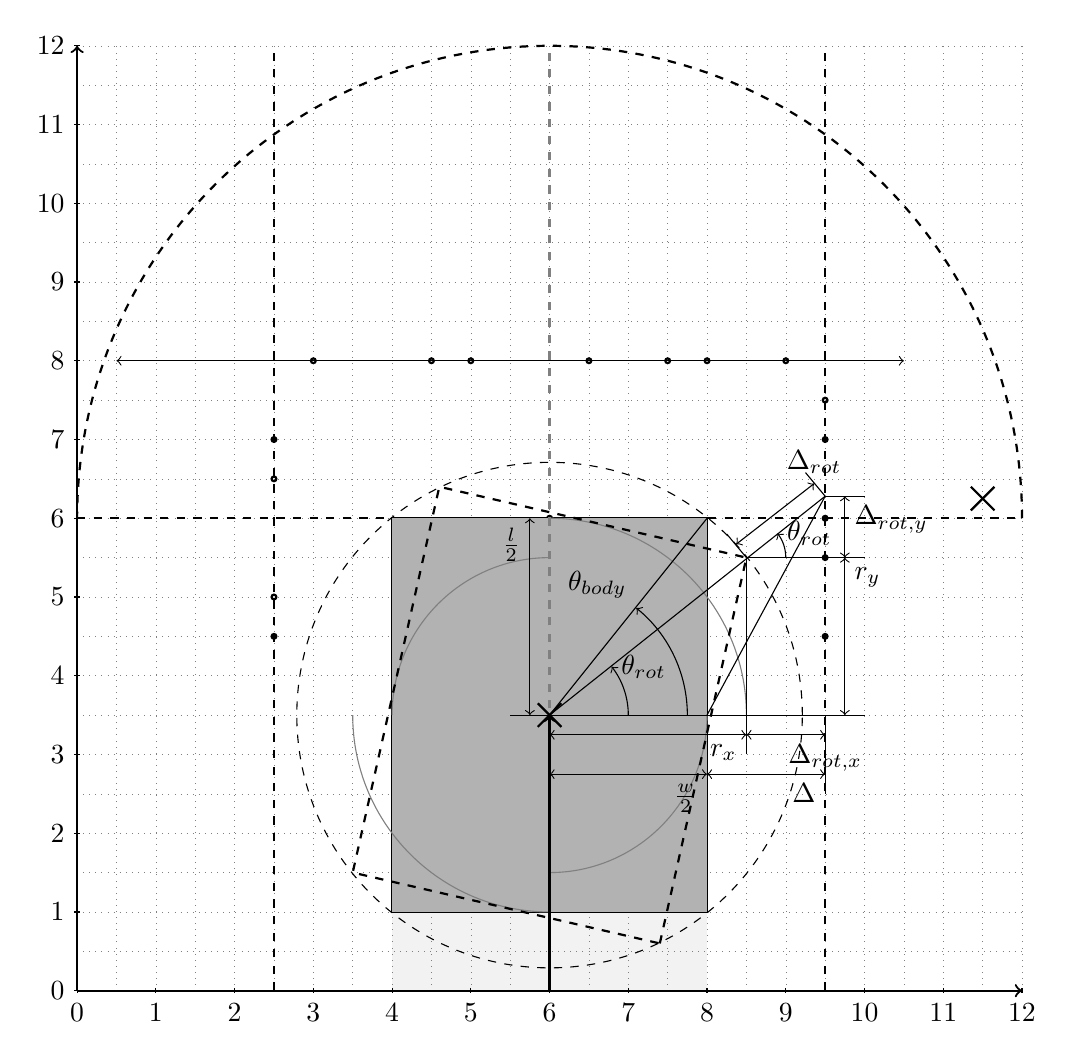
\begin{tikzpicture}
	\fill[black!5!white] (4, 0) -- (8, 0) -- (8, 1) -- (4, 1) -- cycle;
	
	\draw[step = 0.5 cm, gray, very thin, dotted] (0, 0) grid (12, 12);
	\draw[thick, ->] (0, 0) -- (12, 0);
	\draw[thick, ->] (0, 0) -- (0, 12);
	\foreach \x in {0, ..., 12}
	\draw (\x cm, 1 pt) -- (\x cm, -1 pt) node[anchor = north] {$\x$};
	\foreach \y in {0, ..., 12}
	\draw (1 pt, \y cm) -- (-1 pt, \y cm) node[anchor = east] {$\y$};	
	
	\draw[<->] (0.5, 8) -- (10.5, 8);
	
	\draw[thick, dashed] (12, 6) arc (0: 180: 6); 
	\draw[thick, dashed] (2.5, 0) -- (2.5, 12);
	\draw[thick, dashed] (9.5, 0) -- (9.5, 12);
	\draw[thick, dashed] (0, 6) -- (12, 6);
	
	\draw[thick] (4, 1) -- (8, 1) -- (8, 6) -- (4, 6) -- cycle;
	\draw[thick] (6, 6) circle (0.03 cm);
	\fill[black!30!white] (4, 1) rectangle (8, 6);
	
	\draw[gray, thin] (4, 3.5) arc (180:90:2);
	\draw[gray, thin] (8, 3.5) arc (0:-90:2);
	\draw[gray, thin] (8.5, 3.5) arc (0:90:2.5);
	\draw[gray, thin] (6, 1) arc (270:180:2.5);
	
	\draw[thin, dashed] (6, 3.5) circle (3.21);
	
	\draw[thick, dashed] (7.4, 0.6) -- (8.5, 5.5) -- (4.6, 6.4) -- (3.5, 1.5) -- cycle;
	
	\draw[gray, thick, dashed] (6, 0) -- (6, 12);
	
	\draw[thick] (5.85, 3.35) -- (6.15, 3.65);
	\draw[thick] (5.85, 3.65) -- (6.15, 3.35);
	
	\draw[thick] (11.35, 6.1) -- (11.65, 6.4);
	\draw[thick] (11.35, 6.4) -- (11.65, 6.1);
	
	\draw[thick, ->] (6, 0) -- (6, 3.5);
	
	\draw[thick] (3, 8) circle (0.03 cm);
	\draw[thick] (4.5, 8) circle (0.03 cm);
	\draw[thick] (5, 8) circle (0.03 cm);
	\draw[thick] (6.5, 8) circle (0.03 cm);
	\draw[thick] (7.5, 8) circle (0.03 cm);
	\draw[thick] (8, 8) circle (0.03 cm);
	\draw[thick] (9, 8) circle (0.03 cm);
	\draw[thick] (9.5, 7.5) circle (0.03 cm);
	\draw[thick] (9.5, 7) circle (0.03 cm);
	\draw[thick] (9.5, 6) circle (0.03 cm);
	\draw[thick] (9.5, 5.5) circle (0.03 cm);
	\draw[thick] (2.5, 7) circle (0.03 cm);
	\draw[thick] (2.5, 6.5) circle (0.03 cm);
	\draw[thick] (2.5, 5) circle (0.03 cm);
	\draw[thick] (2.5, 4.5) circle (0.03 cm);
	\draw[thick] (9.5, 4.5) circle (0.03 cm);
	
	\draw[thin] (6, 3.5) -- (9.5, 6.28);
	\draw[thin] (6, 3.5) -- (8, 6);
	\draw[thin] (6, 3.5) -- (9.5, 3.5);
	
	\draw[thin] (8.5, 5.5) -- (8.25, 5.8);
	\draw[thin] (9.5, 6.28) -- (9.25, 6.58);
	\draw[thin] (8.5, 3.5) -- (8.5, 5.5);
	\draw[thin, <->] (8.37, 5.67) -- (9.36, 6.44) node[anchor = south] {$\Delta_{rot}$};
	
	\draw[thin, ->] (7, 3.5) arc (0:38:1) node[anchor = west] {$\theta_{rot}$};
	\draw[thin, ->] (7.75, 3.5) arc (0:51:1.75) node[anchor = south east] {$\theta_{body}$};
	\draw[thin] (8.5, 5.5) -- (9.5, 5.5);
	
	\draw[thin, ->] (9, 5.5) arc (0:38:0.5) node[anchor = west] {$\theta_{rot}$};
	
	\draw[thin] (8.5, 3) -- (8.5, 3.5);
	\draw[thin] (9.5, 2.5) -- (9.5, 3.5);
	\draw[thin, <->] (8.5, 3.25) -- (9.5, 3.25) node[anchor = north] {$\Delta_{rot, x}$};
	\draw[thin, <->] (6, 3.25) -- (8.5, 3.25) node[anchor = north east] {$r_{x}$};
	\draw[thin, <->] (6, 2.75) -- (8, 2.75) node[anchor = north east] {$\frac{w}{2}$};
	\draw[thin, <->] (8, 2.75) -- (9.5, 2.75) node[anchor = north east] {$\Delta$};
	\draw[thin] (9.5, 6.28) -- (10, 6.28);
	\draw[thin] (9.5, 5.5) -- (10, 5.5);
	\draw[thin, <->] (9.75, 5.5) -- (9.75, 6.28) node[anchor = north west] {$\Delta_{rot, y}$};
	\draw[thin] (9.5, 3.5) -- (10, 3.5);
	\draw[thin, <->] (9.75, 3.5) -- (9.75, 5.5) node[anchor = north west] {$r_{y}$};
	\draw[thin] (5.5, 3.5) -- (6, 3.5);
	\draw[thin, <->] (5.75, 3.5) -- (5.75, 6) node[anchor = north east] {$\frac{l}{2}$};
	\draw[thin] (8, 3.5) -- (9.5, 6.28);
 	\end{tikzpicture}
 	
 	\begin{align}
 	r \cos \left({\theta_{rot}}\right) &= \frac{w}{2} \\
 	r \sin \left(\theta_{rot}\right) &= \frac{l}{2} \\
 	r &= \sqrt{\left(\frac{l}{2}\right)^{2} + \left(\frac{w}{2}\right)^{2}} \\
 	\implies r &= \frac{1}{2} \sqrt{l^{2} + w^{2}} \\
 	\frac{w}{2} + \Delta &\ge  r + \Delta_{min} \\
 	\implies \Delta &\ge \frac{1}{2} \sqrt{l^{2} + w^{2}} + \Delta_{min} - \frac{w}{2} \\
 	\left(r + \Delta_{rot}\right) \cos \left(\theta_{rot}\right) &= \frac{w}{2} + \Delta \\
 	\cos \left(\theta_{rot}\right) &= \left(\frac{\frac{w}{2} + \Delta}{r + \Delta_{rot}}\right) \\
 	\sin \left(\theta_{rot}\right) &= \sqrt{1 - \left(\frac{\frac{w}{2} + \Delta}{r + \Delta_{rot}}\right)^{2}} \\
 	&= \frac{\sqrt{\left(r + \Delta_{rot}\right)^{2} - \left(\frac{w}{2} + \Delta\right)^{2}}}{r + \Delta_{rot}} \\
 	&= \frac{\sqrt{r^{2} + 2 r \Delta_{rot} + \Delta_{rot}^{2} - \left(\frac{w}{2}\right)^{2} - 2 \left(\frac{w}{2}\right) - \Delta^{2}}}{r + \Delta_{rot}} \\
 	&= \frac{\sqrt{\left(\frac{l}{2}\right)^{2} + \left(\frac{w}{2}\right)^{2} + 2 r \Delta_{rot} + \Delta_{rot}^{2} - \left(\frac{w}{2}\right)^{2} - w - \Delta^{2}}}{r + \Delta_{rot}} \\
 	&= \frac{\sqrt{\left(\frac{l}{2}\right)^{2} + 2 r \Delta_{rot} + \Delta_{rot}^{2} - w - \Delta^{2}}}{r + \Delta_{rot}} \\
 	\implies \left(r + \Delta_{rot}\right) \sin \left(\theta_{rot}\right) &= \sqrt{\left(\frac{l}{2}\right)^{2} + 2 r \Delta_{rot} + \Delta_{rot}^{2} - w - \Delta^{2}} \\
 	&= \sqrt{\frac{l^{2}}{4} + 2 r \Delta_{rot} + \Delta_{rot}^{2} - w - \Delta^{2}} \\
 	y_{gap} &= \left(r + \Delta_{rot}\right) \sin \left(\theta_{rot}\right) \\
 	&= \sqrt{\frac{l^{2}}{4} + 2 r \Delta_{rot} + \Delta_{rot}^{2} - w - \Delta^{2}} \\
 	y_{gap} &\ge \sqrt{\frac{l^{2}}{4} + 2 r \Delta_{min} + \Delta_{min}^{2} - w - \Delta^{2}} \\
 	y_{gap} &\ge \frac{w}{2} + \Delta_{min}
 	\end{align}
 	
 	\begin{align}
 	\Delta &= r_{gap} \cos \left({\theta_{gap}}\right) \\
 	\implies y_{gap} &\ge \sqrt{\frac{l^{2}}{4} + 2 r \Delta_{min} + \Delta_{min}^{2} - w - r_{gap}^{2} \cos^{2} \left({\theta_{gap}}\right)} \\
 	\implies y_{gap} &\ge \sqrt{\frac{l^{2}}{4} + \Delta_{min} \sqrt{l^{2} + w^{2}} + \Delta_{min}^{2} - w - r_{gap}^{2} \cos^{2} \left({\theta_{gap}}\right)}
 	\end{align}
 	
 	\begin{algorithm}[H]
 		\SetAlgoLined
 		\KwResult{$r$ if right rotation is possible, $l$ if left rotation is possible, $none$ if rotation is not possible}
 		compute $C_{right} = \sqrt{\frac{l^{2}}{4} + \Delta_{min} \sqrt{l^{2} + w^{2}} + \Delta_{min}^{2} - w - r_{right, gap}^{2} \cos^{2} \left({\theta_{right, gap}}\right)}$\;
 		compute $C_{left} = \sqrt{\frac{l^{2}}{4} + \Delta_{min} \sqrt{l^{2} + w^{2}} + \Delta_{min}^{2} - w - r_{left, gap}^{2} \cos^{2} \left({\theta_{left, gap}}\right)}$\;
 		compute $y_{right, gap} = r_{right, gap} \sin{\left({\theta_{right, gap}}\right)}$\;
 		compute $y_{left, gap} = r_{left, gap} \sin{\left({\theta_{left, gap}}\right)}$\;
 		compute $y_{gap, min} = \left(\frac{w}{2} + \Delta_{min}\right)$\;
		\eIf{$y_{right, gap} \ge \max \left(C_{right}, y_{gap, min}\right)$}{
			return $r$\;
		}{
			\eIf{$y_{left, gap} \ge \max \left({C_{left}, y_{gap, min}}\right)$}{
				return $l$\;
			}{
				return $none$\;
			}
		}
 \caption{Find rotation direction}
 	\end{algorithm}
 
	 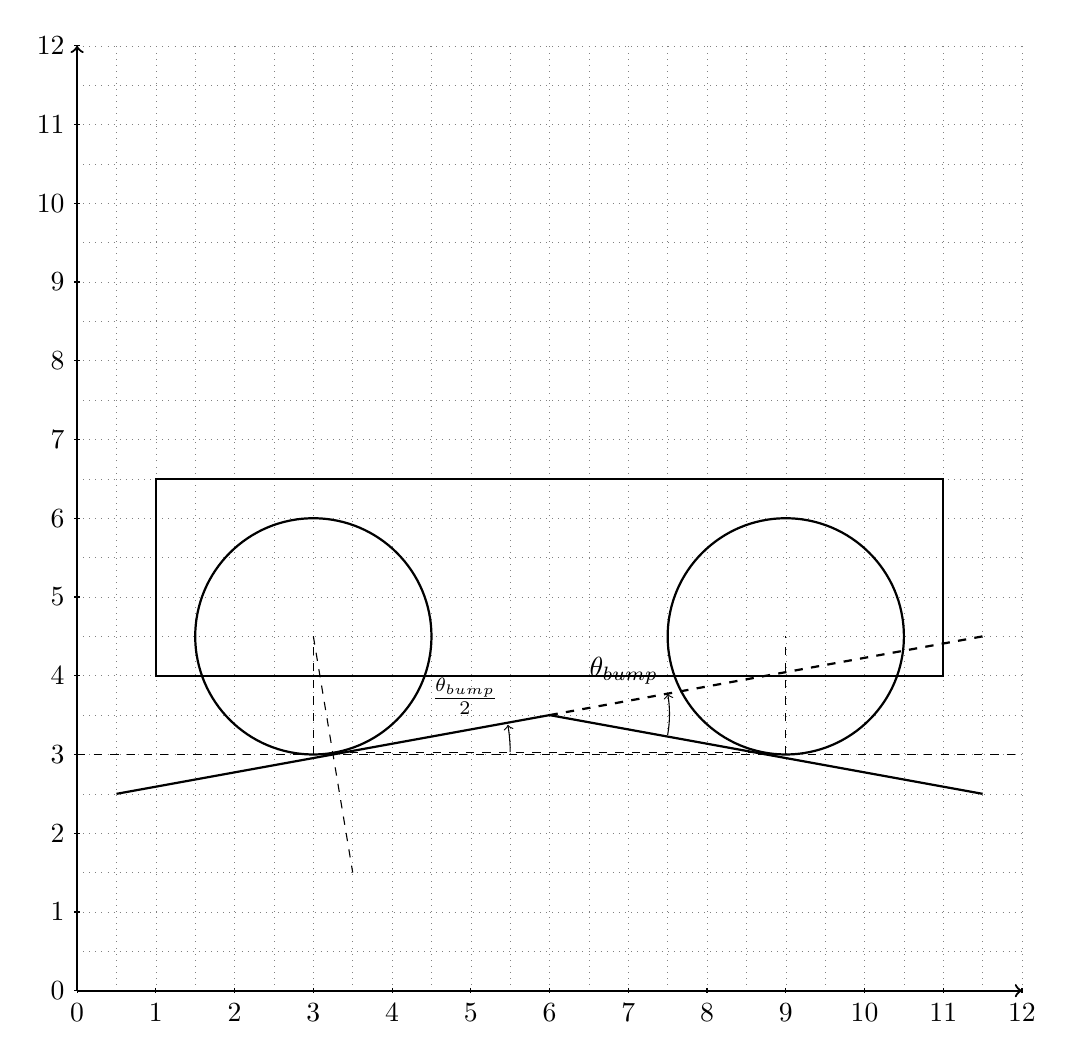
\begin{tikzpicture}
	 \draw[step = 0.5 cm, gray, very thin, dotted] (0, 0) grid (12, 12);
	 \draw[thick, ->] (0, 0) -- (12, 0);
	 \draw[thick, ->] (0, 0) -- (0, 12);
	 \foreach \x in {0, ..., 12}
	 \draw (\x cm, 1 pt) -- (\x cm, -1 pt) node[anchor = north] {$\x$};
	 \foreach \y in {0, ..., 12}
	 \draw (1 pt, \y cm) -- (-1 pt, \y cm) node[anchor = east] {$\y$};	
	 
	 \draw[thick] (1, 4) -- (11, 4) -- (11, 6.5) -- (1, 6.5) -- cycle;
	 
	 \draw[thick] (3, 4.5) circle (1.5);
	 
	 \draw[thick] (9, 4.5) circle (1.5);
	 
	 \draw[thick] (0.5, 2.5) -- (6, 3.5) -- (11.5, 2.5);
	 \draw[thick, dashed] (6, 3.5) -- (11.5, 4.5);
	 
	 \draw[thin, ->] (7.5, 3.25) arc (-10:10:1.5) node[anchor = south east] {$\theta_{bump}$};
	 \draw[thin, dashed] (0, 3) -- (12, 3);
	 
	 \draw[thin, ->] (5.5, 3.03) arc (0:10:2) node[anchor = south east] {$\frac{\theta_{bump}}{2}$};
	 
	 \draw[thin, dashed] (3, 3) -- (3, 4.5);
	 \draw[thin, dashed] (3, 4.5) -- (3.5, 1.5);
	 
	 \draw[thin, dashed] (9, 3) -- (9, 4.5);
	 
	 \draw[thin, dashed] (3.25, 3.03) -- (8.75, 3.03);
	 \end{tikzpicture}
	 
	 \begin{align}
	 	r \cos \left({\frac{\theta_{bump}}{2}}\right) &= \left(r - h\right) + \Delta_{h, min} + p \\
	 	\implies p &= r \cos \left({\frac{\theta_{bump}}{2}}\right) - r + h - \Delta_{h, min} \\
	 	r \sin \left({\frac{\theta_{bump}}{2}}\right) + q &= \frac{d}{2} \\
	 	\implies q &= \frac{d}{2}  - r \sin \left({\frac{\theta_{bump}}{2}}\right) \\
	 	\tan \left({\frac{\theta_{bump}}{2}}\right) &= \frac{p}{q} \\
	 	\implies \tan \left({\frac{\theta_{bump}}{2}}\right) &= \frac{r \cos \left({\frac{\theta_{bump}}{2}}\right) - r + h - \Delta_{h, min}}{\frac{d}{2}  - r \sin \left({\frac{\theta_{bump}}{2}}\right)} \\
	 	\left(\frac{d}{2}  - r \sin \left({\frac{\theta_{bump}}{2}}\right)\right) \tan \left({\frac{\theta_{bump}}{2}}\right) &=  r \cos \left({\frac{\theta_{bump}}{2}}\right) - r + h - \Delta_{h, min} \\
	 	\left(\frac{d}{2}  - r \sin \left({\frac{\theta_{bump}}{2}}\right)\right) \frac{\sin \left({\frac{\theta_{bump}}{2}}\right)}{\cos \left({\frac{\theta_{bump}}{2}}\right)} &=  r \cos \left({\frac{\theta_{bump}}{2}}\right) - r + h - \Delta_{h, min} \\
	 	\left(\frac{d}{2}\right) \sin \left({\frac{\theta_{bump}}{2}}\right)  - r \sin^{2} \left({\frac{\theta_{bump}}{2}}\right) &=  r \cos^{2} \left({\frac{\theta_{bump}}{2}}\right) + \left(- r + h - \Delta_{h, min}\right) \cos \left({\frac{\theta_{bump}}{2}}\right) \\
	 	\implies \left(\frac{d}{2}\right) \sin \left({\frac{\theta_{bump}}{2}}\right) &=  r \cos^{2} \left({\frac{\theta_{bump}}{2}}\right) + r \sin^{2} \left({\frac{\theta_{bump}}{2}}\right) + \left(- r + h - \Delta_{h, min}\right) \cos \left({\frac{\theta_{bump}}{2}}\right) \\
	 	\left(\frac{d}{2}\right) \sin \left({\frac{\theta_{bump}}{2}}\right) &=  r \left(\cos^{2} \left({\frac{\theta_{bump}}{2}}\right) + \sin^{2} \left({\frac{\theta_{bump}}{2}}\right)\right) + \left(- r + h - \Delta_{h, min}\right) \cos \left({\frac{\theta_{bump}}{2}}\right) \\
	 	\left(\frac{d}{2}\right) \sin \left({\frac{\theta_{bump}}{2}}\right) &=  r + \left(- r + h - \Delta_{h, min}\right) \cos \left({\frac{\theta_{bump}}{2}}\right) \\
	 	\left(\left(\frac{d}{2}\right) \sin \left({\frac{\theta_{bump}}{2}}\right)\right)^{2} &=  \left(r + \left(- r + h - \Delta_{h, min}\right) \cos \left({\frac{\theta_{bump}}{2}}\right)\right)^{2} \\
	 	\left(\frac{d}{2}\right)^{2} \sin^{2} \left({\frac{\theta_{bump}}{2}}\right) &=  r^{2} + 2 r \left(- r + h - \Delta_{h, min}\right) \cos \left({\frac{\theta_{bump}}{2}}\right) + \left(- r + h - \Delta_{h, min}\right)^{2} \cos^{2} \left({\frac{\theta_{bump}}{2}}\right)
	 \end{align}
	 
	 \begin{align}
	 r^{2} + 2 r \left(- r + h - \Delta_{h, min}\right) \cos \left({\frac{\theta_{bump}}{2}}\right) + \left(- r + h - \Delta_{h, min}\right)^{2} \cos^{2} \left({\frac{\theta_{bump}}{2}}\right) - \left(\frac{d}{2}\right)^{2} \sin^{2} \left({\frac{\theta_{bump}}{2}}\right) &= 0 \\
	 r^{2} + 2 r \left(- r + h - \Delta_{h, min}\right) \cos \left({\frac{\theta_{bump}}{2}}\right) + \left(- r + h - \Delta_{h, min}\right)^{2} \cos^{2} \left({\frac{\theta_{bump}}{2}}\right) - \left(\frac{d}{2}\right)^{2} \left(1 - \cos^{2} \left({\frac{\theta_{bump}}{2}}\right)\right) &= 0 \\
	 r^{2} + 2 r \left(- r + h - \Delta_{h, min}\right) \cos \left({\frac{\theta_{bump}}{2}}\right) + \left(- r + h - \Delta_{h, min}\right)^{2} \cos^{2} \left({\frac{\theta_{bump}}{2}}\right) - \left(\frac{d}{2}\right)^{2} + \left(\frac{d}{2}\right)^{2} \cos^{2} \left({\frac{\theta_{bump}}{2}}\right) &= 0 \\
	 \left(\left(\frac{d}{2}\right)^{2} + \left(- r + h - \Delta_{h, min}\right)^{2}\right) \cos^{2} \left({\frac{\theta_{bump}}{2}}\right) + 2 r \left(- r + h - \Delta_{h, min}\right) \cos \left({\frac{\theta_{bump}}{2}}\right) + r^{2} - \left(\frac{d}{2}\right)^{2} &= 0
	 \end{align}
	 
	 \begin{align}
	 \cos \left({\frac{\theta_{bump}}{2}}\right) &= \frac{- 2 r \left(- r + h - \Delta_{h, min}\right) \pm \sqrt{\left(2 r \left(- r + h - \Delta_{h, min}\right)\right)^{2} - 4 \left(\left(\frac{d}{2}\right)^{2} + \left(- r + h - \Delta_{h, min}\right)^{2}\right) \left(r^{2} - \left(\frac{d}{2}\right)^{2}\right)}}{2 \left(\left(\frac{d}{2}\right)^{2} + \left(- r + h - \Delta_{h, min}\right)^{2}\right)} \\
	 \implies {\frac{\theta_{bump}}{2}} &= \cos^{-1} \left(\frac{- 2 r \left(- r + h - \Delta_{h, min}\right) \pm \sqrt{\left(2 r \left(- r + h - \Delta_{h, min}\right)\right)^{2} - 4 \left(\left(\frac{d}{2}\right)^{2} + \left(- r + h - \Delta_{h, min}\right)^{2}\right) \left(r^{2} - \left(\frac{d}{2}\right)^{2}\right)}}{2 \left(\left(\frac{d}{2}\right)^{2} + \left(- r + h - \Delta_{h, min}\right)^{2}\right)}\right) \\
	 \therefore \theta_{bump} &= 2 \cos^{-1} \left(\frac{- 2 r \left(- r + h - \Delta_{h, min}\right) \pm \sqrt{\left(2 r \left(- r + h - \Delta_{h, min}\right)\right)^{2} - 4 \left(\left(\frac{d}{2}\right)^{2} + \left(- r + h - \Delta_{h, min}\right)^{2}\right) \left(r^{2} - \left(\frac{d}{2}\right)^{2}\right)}}{2 \left(\left(\frac{d}{2}\right)^{2} + \left(- r + h - \Delta_{h, min}\right)^{2}\right)}\right) \\
	 &= 2 \cos^{-1} \left(\frac{- 2 r \left(- r + h - \Delta_{h, min}\right) \pm 2 \sqrt{\left(r \left(- r + h - \Delta_{h, min}\right)\right)^{2} - \left(\left(\frac{d}{2}\right)^{2} + \left(- r + h - \Delta_{h, min}\right)^{2}\right) \left(r^{2} - \left(\frac{d}{2}\right)^{2}\right)}}{2 \left(\left(\frac{d}{2}\right)^{2} + \left(- r + h - \Delta_{h, min}\right)^{2}\right)}\right) \\
	 &= 2 \cos^{-1} \left(\frac{- r \left(- r + h - \Delta_{h, min}\right) \pm \sqrt{\left(r \left(- r + h - \Delta_{h, min}\right)\right)^{2} - \left(\left(\frac{d}{2}\right)^{2} + \left(- r + h - \Delta_{h, min}\right)^{2}\right) \left(r^{2} - \left(\frac{d}{2}\right)^{2}\right)}}{\left(\left(\frac{d}{2}\right)^{2} + \left(- r + h - \Delta_{h, min}\right)^{2}\right)}\right)
	 \end{align}
	 
	 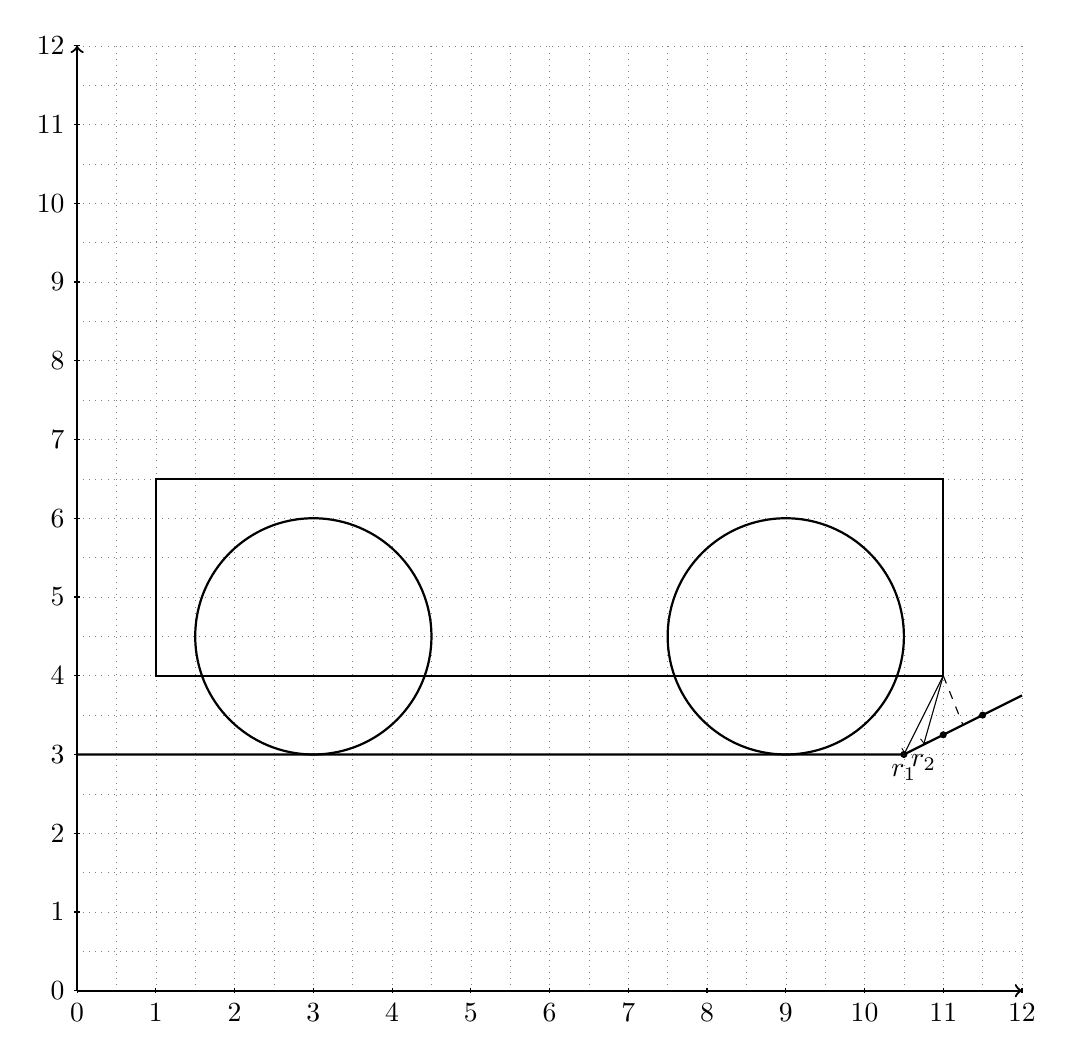
\begin{tikzpicture}
	 \draw[step = 0.5 cm, gray, very thin, dotted] (0, 0) grid (12, 12);
	 \draw[thick, ->] (0, 0) -- (12, 0);
	 \draw[thick, ->] (0, 0) -- (0, 12);
	 \foreach \x in {0, ..., 12}
	 \draw (\x cm, 1 pt) -- (\x cm, -1 pt) node[anchor = north] {$\x$};
	 \foreach \y in {0, ..., 12}
	 \draw (1 pt, \y cm) -- (-1 pt, \y cm) node[anchor = east] {$\y$};	
	 
	 \draw[thick] (1, 4) -- (11, 4) -- (11, 6.5) -- (1, 6.5) -- cycle;
	 
	 \draw[thick] (3, 4.5) circle (1.5);
	 
	 \draw[thick] (9, 4.5) circle (1.5);
	 
	 \draw[thick] (0, 3) -- (10.5, 3) -- (12, 3.75);
	 
	 \draw[thick] (10.5, 3) circle (0.03 cm);
	 \draw[thick] (11, 3.25) circle (0.03 cm);
	 \draw[thick] (11.5, 3.5) circle (0.03 cm);
	 
	 \draw[thin, ->] (11, 4) -- (10.5, 3) node [anchor = north] {$r_{1}$};
	 \draw[thin, ->] (11, 4) -- (10.75, 3.125) node [anchor = north] {$r_{2}$};
	 \draw[thin, dashed] (11, 4) -- (11.25, 3.375);
	 \end{tikzpicture}
	 
	 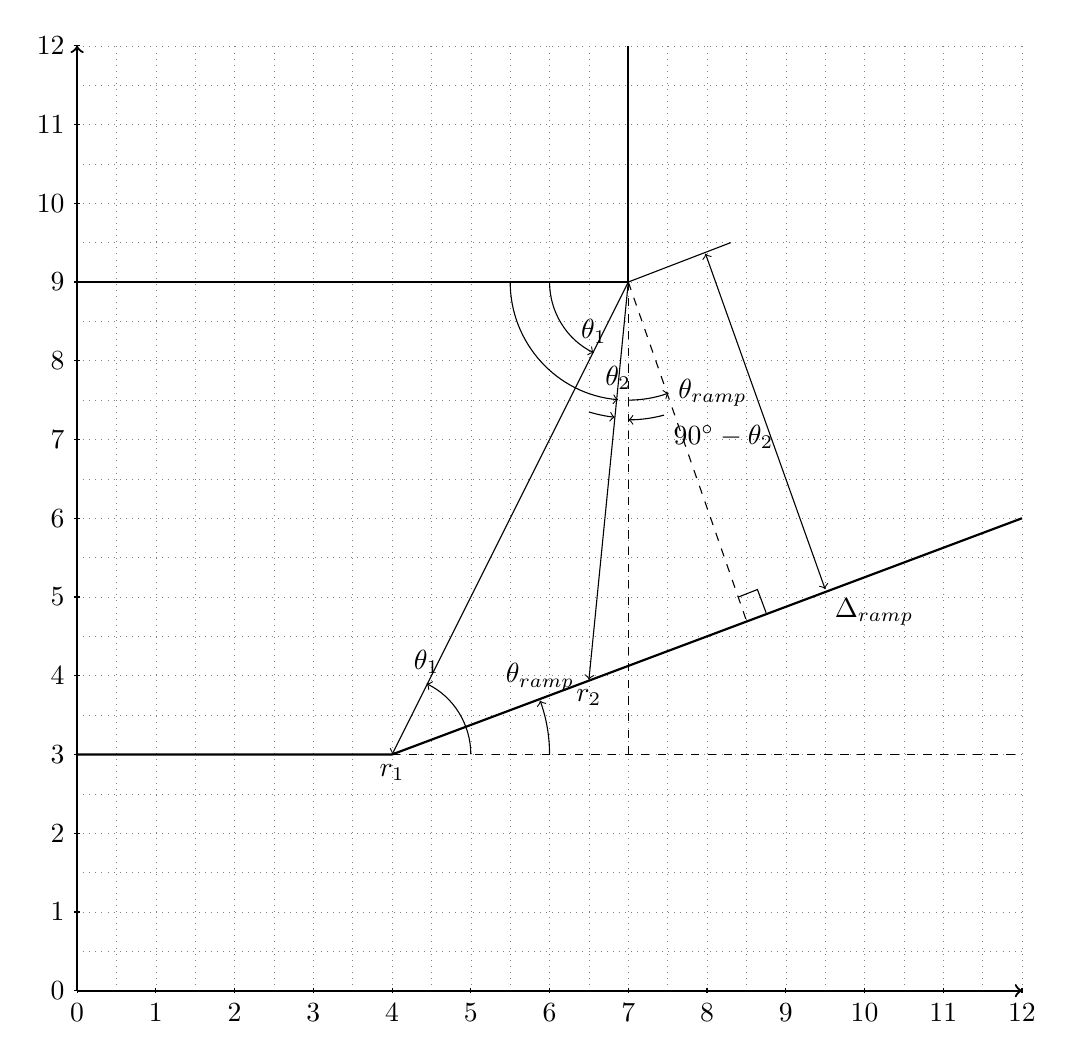
\begin{tikzpicture}
	 \draw[step = 0.5 cm, gray, very thin, dotted] (0, 0) grid (12, 12);
	 \draw[thick, ->] (0, 0) -- (12, 0);
	 \draw[thick, ->] (0, 0) -- (0, 12);
	 \foreach \x in {0, ..., 12}
	 \draw (\x cm, 1 pt) -- (\x cm, -1 pt) node[anchor = north] {$\x$};
	 \foreach \y in {0, ..., 12}
	 \draw (1 pt, \y cm) -- (-1 pt, \y cm) node[anchor = east] {$\y$};	
	 
	 \draw[thick] (0, 3) -- (4, 3) -- (12, 6);
	 \draw[thin, ->] (7, 9) -- (4, 3) node[anchor = north] {$r_{1}$};
	 \draw[thin, ->] (7, 9) -- (6.5, 3.95) node[anchor = north] {$r_{2}$};
	 \draw[thin, dashed] (7, 9) -- (8.5, 4.7);
	 \draw[thick] (0, 9) -- (7, 9) -- (7, 12);
	 \draw[thin, dashed] (4, 3) -- (12, 3);
	 \draw[thin] (8.4, 5) -- (8.64, 5.095) -- (8.75, 4.8);
	 
	 \draw[thin, ->] (6, 3) arc (0:20:2) node[anchor = south] {$\theta_{ramp}$}; 
	 \draw[thin, ->] (6, 9) arc (180:244:1) node[anchor = south] {$\theta_{1}$};
	 \draw[thin, ->] (5.5, 9) arc (180:265:1.5) node[anchor = south] {$\theta_{2}$};
	 \draw[thin, ->] (5, 3) arc (0:64:1) node[anchor = south] {$\theta_{1}$};
	 
	 \draw[thin, dashed] (7, 3) -- (7, 9);
	 
	 \draw[thin, ->] (7, 7.5) arc (270:290:1.5) node[anchor = west] {$\theta_{ramp}$};
	 
	 \draw[thin, ->] (6.5, 7.35) arc (253:264:1.75); 
	 \draw[thin, <-] (7, 7.25) arc (270:285:1.75) node[anchor = north west] {$90^{\circ} - \theta_{2}$};
	 
	 \draw[thin] (7, 9) -- (8.3, 9.5);
	 \draw[thin, <->] (7.98, 9.36) -- (9.5, 5.1) node[anchor = north west] {$\Delta_{ramp}$};
	 \end{tikzpicture}
	 
	 \begin{align}
	 r_{2} \cos \left({90^{\circ} - \theta_{2} + \theta_{ramp}}\right) &= \Delta_{ramp} \\
	 \implies r_{2} \cos \left({90^{\circ} - \left(\theta_{2} - \theta_{ramp}\right)}\right) &= \Delta_{ramp} \\
	 r_{2} \sin \left({\theta_{2} - \theta_{ramp}}\right) &= \Delta_{ramp} \\
	 r_{2} \left(\sin \left({\theta_{2}}\right) \cos \left({\theta_{ramp}}\right) - \cos \left({\theta_{2}}\right) \sin \left({\theta_{ramp}}\right)\right) &= \Delta_{ramp} \\
	 \tan \left({\theta_{ramp}}\right) &= \frac{r_{1} \sin \left(\theta_{1}\right) - r_{2} \sin \left(\theta_{2}\right)}{r_{1} \cos \left(\theta_{1}\right) - r_{2} \cos \left(\theta_{2}\right)} \\
	 \implies \sin \left({\theta_{ramp}}\right) &= \frac{r_{1} \sin \left(\theta_{1}\right) - r_{2} \sin \left(\theta_{2}\right)}{\sqrt{\left(r_{1} \sin \left(\theta_{1}\right) - r_{2} \sin \left(\theta_{2}\right)\right)^{2} + \left(r_{1} \cos \left(\theta_{1}\right) - r_{2} \cos \left(\theta_{2}\right)\right)^{2}}} \\
	 \implies \cos \left({\theta_{ramp}}\right) &= \frac{r_{1} \cos \left(\theta_{1}\right) - r_{2} \cos \left(\theta_{2}\right)}{\sqrt{\left(r_{1} \sin \left(\theta_{1}\right) - r_{2} \sin \left(\theta_{2}\right)\right)^{2} + \left(r_{1} \cos \left(\theta_{1}\right) - r_{2} \cos \left(\theta_{2}\right)\right)^{2}}}
	 \end{align}
	 
	 \begin{align}
	 \therefore r_{2} \frac{\left(\sin \left({\theta_{2}}\right) \left(r_{1} \cos \left(\theta_{1}\right) - r_{2} \cos \left(\theta_{2}\right)\right) - \cos \left({\theta_{2}}\right) \left(r_{1} \sin \left(\theta_{1}\right) - r_{2} \sin \left(\theta_{2}\right)\right)\right)}{\sqrt{\left(r_{1} \sin \left(\theta_{1}\right) - r_{2} \sin \left(\theta_{2}\right)\right)^{2} + \left(r_{1} \cos \left(\theta_{1}\right) - r_{2} \cos \left(\theta_{2}\right)\right)^{2}}} &= \Delta_{ramp} \\
	 r_{2} \frac{\left(\sin \left({\theta_{2}}\right) \left(r_{1} \cos \left(\theta_{1}\right) - r_{2} \cos \left(\theta_{2}\right)\right) - \cos \left({\theta_{2}}\right) \left(r_{1} \sin \left(\theta_{1}\right) - r_{2} \sin \left(\theta_{2}\right)\right)\right)}{\sqrt{\left(r_{1} \sin \left(\theta_{1}\right) - r_{2} \sin \left(\theta_{2}\right)\right)^{2} + \left(r_{1} \cos \left(\theta_{1}\right) - r_{2} \cos \left(\theta_{2}\right)\right)^{2}}} &= \Delta_{ramp} \\
	 r_{2} \frac{\left(\left(r_{1} \sin \left({\theta_{2}}\right) \cos \left(\theta_{1}\right) - r_{2} \sin \left({\theta_{2}}\right) \cos \left(\theta_{2}\right)\right) - \left(r_{1} \sin \left(\theta_{1}\right) \cos \left({\theta_{2}}\right) - r_{2} \sin \left(\theta_{2}\right) \cos \left({\theta_{2}}\right)\right)\right)}{\sqrt{\left(r_{1} \sin \left(\theta_{1}\right) - r_{2} \sin \left(\theta_{2}\right)\right)^{2} + \left(r_{1} \cos \left(\theta_{1}\right) - r_{2} \cos \left(\theta_{2}\right)\right)^{2}}} &= \Delta_{ramp} \\
	 r_{2} \frac{\left(\left(r_{1} \sin \left({\theta_{2}}\right) \cos \left(\theta_{1} - r_{1} \sin \left(\theta_{1}\right) \cos \left({\theta_{2}}\right)\right)\right) - \left(r_{2} \sin \left({\theta_{2}}\right) \cos \left(\theta_{2}\right) - r_{2} \sin \left(\theta_{2}\right) \cos \left({\theta_{2}}\right)\right)\right)}{\sqrt{\left(r_{1} \sin \left(\theta_{1}\right) - r_{2} \sin \left(\theta_{2}\right)\right)^{2} + \left(r_{1} \cos \left(\theta_{1}\right) - r_{2} \cos \left(\theta_{2}\right)\right)^{2}}} &= \Delta_{ramp} \\
	 r_{1} r_{2} \frac{\left(\left(r_{1} \sin \left({\theta_{2}}\right) \cos \left(\theta_{1} - r_{1} \sin \left(\theta_{1}\right) \cos \left({\theta_{2}}\right)\right)\right)\right)}{\sqrt{\left(r_{1} \sin \left(\theta_{1}\right) - r_{2} \sin \left(\theta_{2}\right)\right)^{2} + \left(r_{1} \cos \left(\theta_{1}\right) - r_{2} \cos \left(\theta_{2}\right)\right)^{2}}} &= \Delta_{ramp} \\
	 r_{1} r_{2} \frac{\left(\left( \sin \left({\theta_{2}}\right) \cos \left(\theta_{1}\right) - \sin \left(\theta_{1}\right) \cos \left({\theta_{2}}\right)\right)\right)}{\sqrt{\left(r_{1} \sin \left(\theta_{1}\right) - r_{2} \sin \left(\theta_{2}\right)\right)^{2} + \left(r_{1} \cos \left(\theta_{1}\right) - r_{2} \cos \left(\theta_{2}\right)\right)^{2}}} &= \Delta_{ramp} \\
	 \frac{r_{1} r_{2} \sin \left({\theta_{2} - \theta_{1}}\right)}{\sqrt{\left(r_{1} \sin \left(\theta_{1}\right) - r_{2} \sin \left(\theta_{2}\right)\right)^{2} + \left(r_{1} \cos \left(\theta_{1}\right) - r_{2} \cos \left(\theta_{2}\right)\right)^{2}}} &= \Delta_{ramp} \\
	 \frac{r_{1} r_{2} \sin \left({\theta_{2} - \theta_{1}}\right)}{\sqrt{r_{1}^{2} + r_{2}^{2} - 2 r_{1} r_{2} \cos \left({\theta_{2} - \theta_{1}}\right)}} &= \Delta_{ramp}
	 \end{align}
	 
	 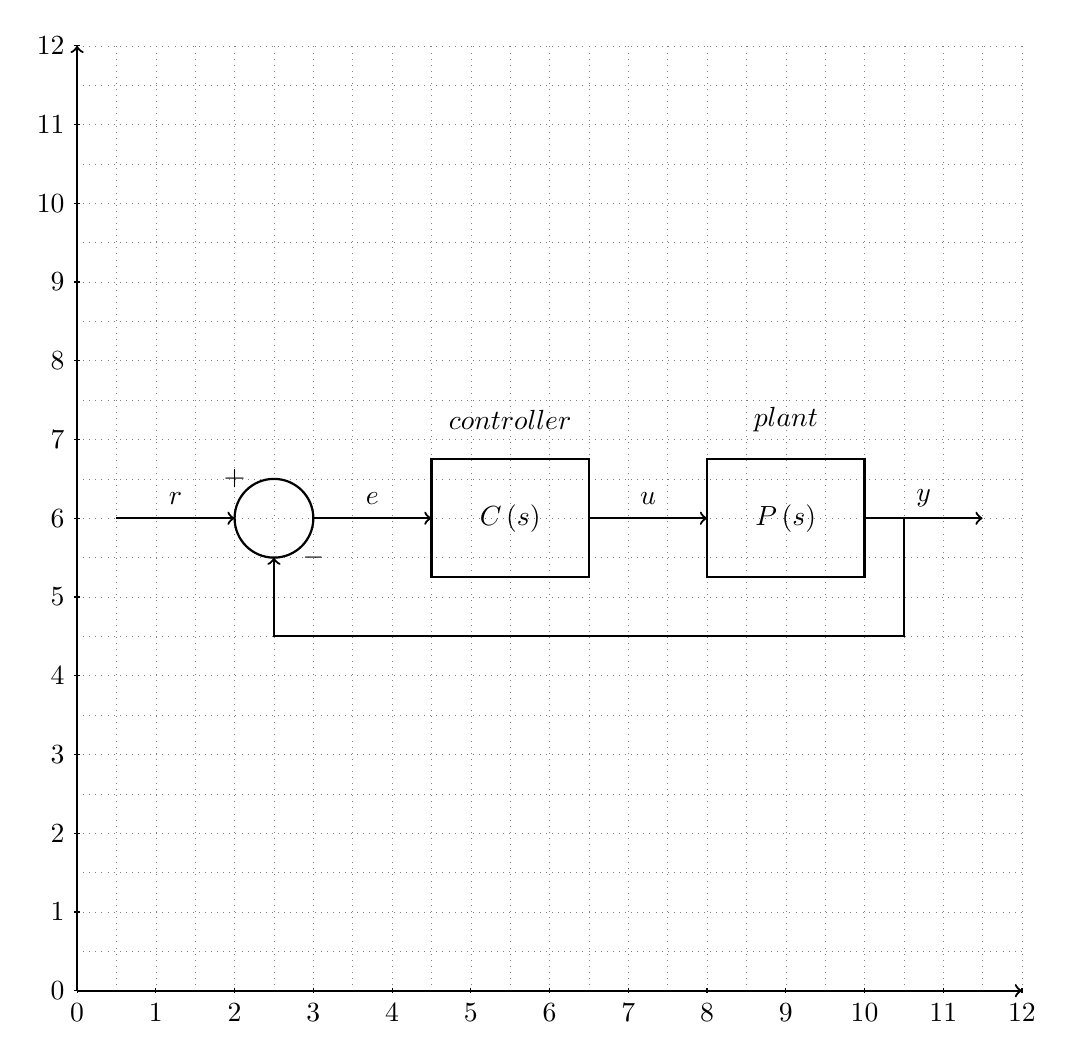
\begin{tikzpicture}
	 \draw[step = 0.5 cm, gray, very thin, dotted] (0, 0) grid (12, 12);
	 \draw[thick, ->] (0, 0) -- (12, 0);
	 \draw[thick, ->] (0, 0) -- (0, 12);
	 \foreach \x in {0, ..., 12}
	 \draw (\x cm, 1 pt) -- (\x cm, -1 pt) node[anchor = north] {$\x$};
	 \foreach \y in {0, ..., 12}
	 \draw (1 pt, \y cm) -- (-1 pt, \y cm) node[anchor = east] {$\y$};	
	 
	 \draw[thick, ->] (0.5, 6) -- (2, 6);
	 \node[align = center] at (1.25, 6.25) {$r$};	 
	 
	 \draw[thick] (2.5, 6) circle (0.5);
	 
	  \draw[thick, ->] (3, 6) -- (4.5, 6);
	  \node[align = center] at (3.75, 6.25) {$e$};
	  
	  \draw[thick] (4.5, 6.75) rectangle (6.5, 5.25);
	  
	  \draw[thick, ->] (6.5, 6) -- (8, 6);
	  \node[align = center] at (7.25, 6.25) {$u$};
	  
	  \draw[thick] (8, 6.75) rectangle (10, 5.25);
	  
	  \draw[thick, ->] (10, 6) -- (11.5, 6);
	  \node[align = center] at (10.75, 6.25) {$y$};
	  
	  \draw[thick, <-] (2.5, 5.5) -- (2.5, 4.5) -- (10.5, 4.5) -- (10.5, 6);
	  
	  \node[align = center] at (5.5, 6) {$C\left(s\right)$};
	  
	  \node[align = center] at (9, 6) {$P\left(s\right)$};
	  
	  \node[align = center] at (5.5, 7.25) {$controller$};
	  
	  \node[align = center] at (9, 7.25) {$plant$};
	  
	  \node[align = center] at (2, 6.5) {$+$};
	  
	  \node[align = center] at (3, 5.5) {$-$};
	 \end{tikzpicture}
	 
	 \begin{align}
	 	u\left(t\right) &= K_{p} e\left(t\right) + K_{i} \int e\left(t\right) dt + K_{d} \frac{de\left(t\right)}{dt}
	 \end{align}
	 
	 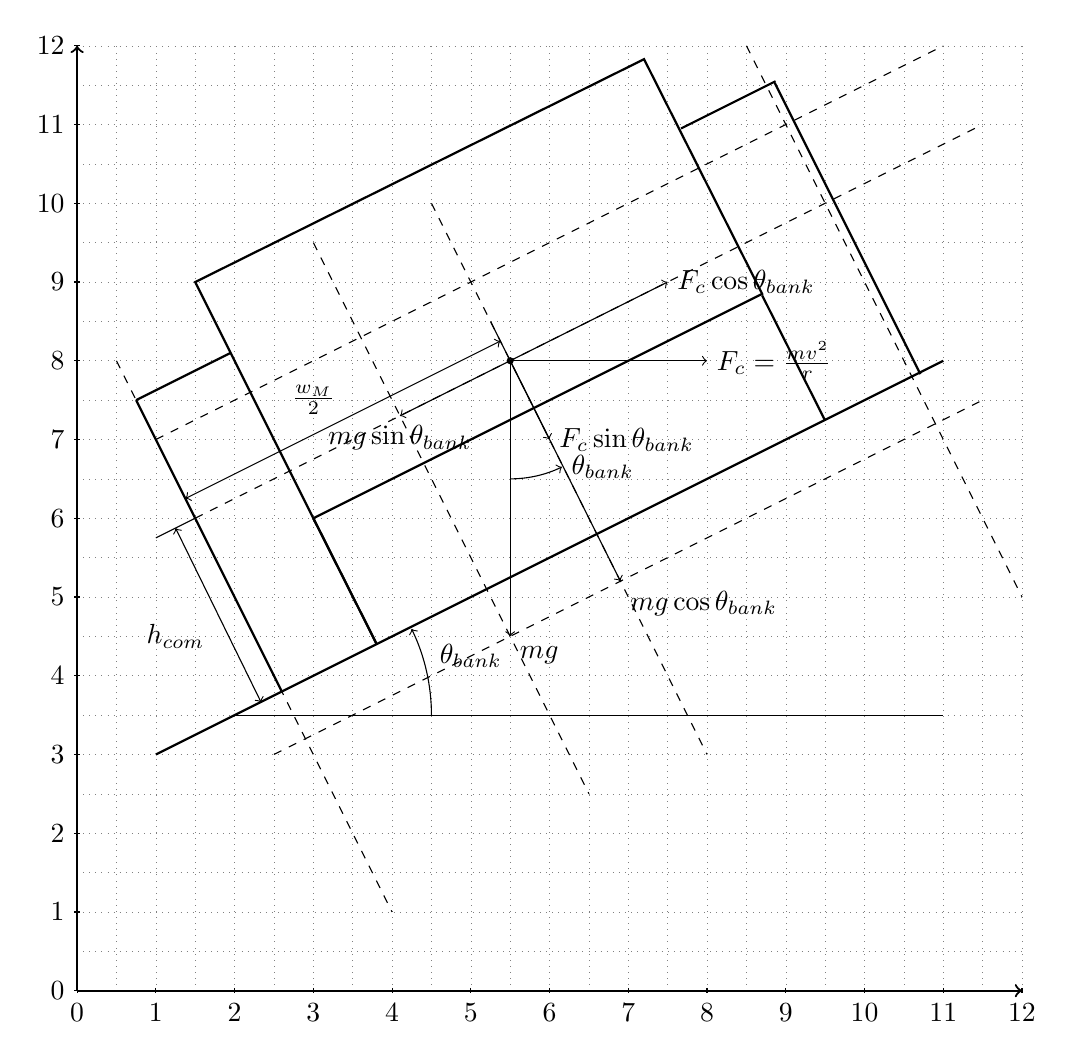
\begin{tikzpicture}
	 \draw[step = 0.5 cm, gray, very thin, dotted] (0, 0) grid (12, 12);
	 \draw[thick, ->] (0, 0) -- (12, 0);
	 \draw[thick, ->] (0, 0) -- (0, 12);
	 \foreach \x in {0, ..., 12}
	 \draw (\x cm, 1 pt) -- (\x cm, -1 pt) node[anchor = north] {$\x$};
	 \foreach \y in {0, ..., 12}
	 \draw (1 pt, \y cm) -- (-1 pt, \y cm) node[anchor = east] {$\y$};
	 
	 \draw[thick] (1, 3) -- (11, 8);
	 
	 \draw[thin, dashed] (1, 7) -- (11, 12);
	 
	 \draw[thin, dashed] (0.5, 8) -- (4, 1);
	 
	 \draw[thin, dashed] (4.5, 10) -- (8, 3);
	 
	 \draw[thin, dashed] (8.5, 12) -- (12, 5);
	 
	 \draw[thick] (1.5, 9) -- (3, 6) -- (8.7, 8.85) -- (7.2, 11.83) -- cycle;
	 
	 \draw[thick] (5.5, 8) circle (0.03 cm);
	 
	 \draw[thin, ->] (5.5, 8) -- (5.5, 4.5) node[anchor = north west] {$mg$};
	 
	 \draw[thin] (2, 3.5) -- (11, 3.5);
	 
	 \draw[thin, dashed] (1.5, 6) -- (11.5, 11);
	 \draw[thin, dashed] (3, 9.5) -- (6.5, 2.5);
	 \draw[thin, dashed] (2.5, 3) -- (11.5, 7.5);
	 
	 \draw[thin, ->] (5.5, 8) -- (4.1, 7.3) node[anchor = north] {$mg \sin \theta_{bank}$};
	 \draw[thin, ->] (5.5, 8) -- (6.9, 5.2) node[anchor = north west] {$mg \cos \theta_{bank} $};
	 
	 \draw[thin, ->] (5.5, 8) -- (8, 8) node[anchor = west] {$F_{c} = \frac{m v^{2}}{r}$};
	 \draw[thin, ->] (4.5, 3.5) arc (0:26:2.5);
	 
	 \node[align = center] at (5, 4.25) {$\theta_{bank}$};
	 
	 \draw[thin, ->] (5.5, 6.5) arc (270:296:1.5) node[anchor = west] {$\theta_{bank}$};
	 
	 \draw[thin] (1.5, 6) -- (1.25, 6.5);
	 \draw[thin] (5.5, 8) -- (5.25, 8.5);
	 \draw[thin, <->] (1.375, 6.25) -- (5.375, 8.25);
	 
	 \node[align = center] at (3, 7.5) {$\frac{w_{M}}{2}$};
	 
	 \draw[thin] (1, 5.75) -- (1.5, 6);
	 \draw[thin, <->] (1.25, 5.875) -- (2.338, 3.66);
	 
	 \node[align = center] at (1.25, 4.5) {$h_{com}$};
	 
	 \draw[thin, ->] (5.5, 8) -- (7.5, 9) node[anchor = west] {$F_{c} \cos {\theta_{bank}}$};
	 \draw[thin, ->] (5.5, 8) -- (6, 7) node[anchor = west] {$F_{c} \sin {\theta_{bank}}$};
	 
	 \draw[thick] (0.75, 7.5) -- (1.95, 8.1);
	 \draw[thick] (0.75, 7.5) -- (2.6, 3.8);
	 \draw[thick] (3, 6) -- (3.8, 4.41);
	 
	 \draw[thick] (7.67, 10.95) -- (8.87, 11.55);
	 \draw[thick] (8.86, 11.53) -- (10.71, 7.83);
	 \draw[thick] (3, 6) -- (3.8, 4.41);
	 \draw[thick] (8.7, 8.83) -- (9.5, 7.24);
	 \end{tikzpicture}
	 
	 \begin{align}
	 \left(m g \cos \theta_{bank} + F_{c} \sin \theta_{bank}\right) \frac{w_{M}}{2} &= \left(m g \sin \theta_{bank} - F_{c} \cos \theta_{bank}\right) h_{com} \\
	 \left(m g + F_{c} \tan \theta_{bank}\right) \frac{w_{M}}{2} &= \left(m g \tan \theta_{bank} - F_{c}\right) h_{com} \\
	 m g h_{com} \tan \theta_{bank} - F_{c} \frac{w_{M}}{2} \tan \theta_{bank} &= m g \frac{w_{M}}{2} + F_{c} h_{com} \\
	 \left(m g h_{com} - F_{c} \frac{w_{M}}{2} \right) \tan \theta_{bank} &= m g \frac{w_{M}}{2} + F_{c} h_{com} \\
	 \tan \theta_{bank} &= \frac{m g \frac{w_{M}}{2} + F_{c} h_{com}}{m g h_{com} - F_{c} \frac{w_{M}}{2}} \\
	 \theta_{bank} &= \tan^{-1} \left(\frac{m g \frac{w_{M}}{2} + F_{c} h_{com}}{m g h_{com} - F_{c}}\right) \\
	 \theta_{bank} &= \tan^{-1} \left(\frac{m g \frac{w_{M}}{2} + \frac{m v^{2}}{r} h_{com}}{m g h_{com} - \frac{m v^{2}}{r}}\right)
	 \end{align}
	 
	 \begin{align}
	 \theta_{bank} &= \lim_{r \rightarrow \infty} \left(\tan^{-1} \left(\frac{m g \frac{w_{M}}{2} + \frac{m v^{2}}{r} h_{com}}{m g h_{com} - \frac{m v^{2}}{r}}\right)\right) &= \tan^{-1} \left(\frac{m g \frac{w_{M}}{2}}{m g h_{com}}\right) \\
	 &= \tan^{-1} \left(\frac{w_{M}}{2 h_{com}}\right)
	 \end{align}
	 
	 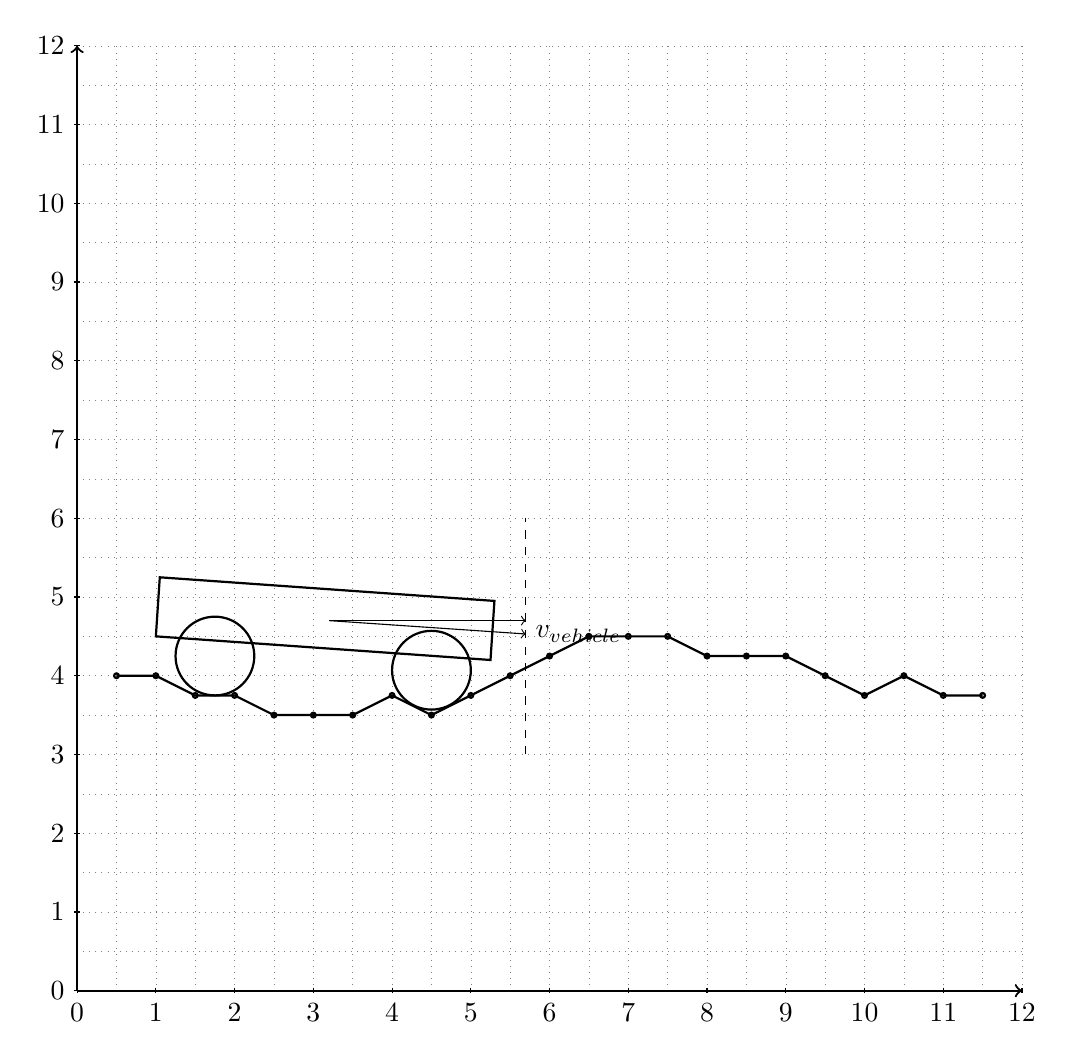
\begin{tikzpicture}
	 \draw[step = 0.5 cm, gray, very thin, dotted] (0, 0) grid (12, 12);
	 \draw[thick, ->] (0, 0) -- (12, 0);
	 \draw[thick, ->] (0, 0) -- (0, 12);
	 \foreach \x in {0, ..., 12}
	 \draw (\x cm, 1 pt) -- (\x cm, -1 pt) node[anchor = north] {$\x$};
	 \foreach \y in {0, ..., 12}
	 \draw (1 pt, \y cm) -- (-1 pt, \y cm) node[anchor = east] {$\y$};
	 
	 \draw[thick] (0.5, 4) circle (0.03 cm);
	 \draw[thick] (1, 4) circle (0.03 cm);
	 \draw[thick] (1.5, 3.75) circle (0.03 cm);
	 \draw[thick] (2, 3.75) circle (0.03 cm);
	 \draw[thick] (2.5, 3.5) circle (0.03 cm);
	 \draw[thick] (3, 3.5) circle (0.03 cm);
	 \draw[thick] (3.5, 3.5) circle (0.03 cm);
	 \draw[thick] (4, 3.75) circle (0.03 cm);
	 \draw[thick] (4.5, 3.5) circle (0.03 cm);
	 \draw[thick] (5, 3.75) circle (0.03 cm);
	 \draw[thick] (5.5, 4) circle (0.03 cm);
	 \draw[thick] (6, 4.25) circle (0.03 cm);
	 \draw[thick] (6.5, 4.5) circle (0.03 cm);
	 \draw[thick] (7, 4.5) circle (0.03 cm);
	 \draw[thick] (7.5, 4.5) circle (0.03 cm);
	 \draw[thick] (8, 4.25) circle (0.03 cm);
	 \draw[thick] (8.5, 4.25) circle (0.03 cm);
	 \draw[thick] (9, 4.25) circle (0.03 cm);
	 \draw[thick] (9.5, 4) circle (0.03 cm);
	 \draw[thick] (10, 3.75) circle (0.03 cm);
	 \draw[thick] (10.5, 4) circle (0.03 cm);
	 \draw[thick] (11, 3.75) circle (0.03 cm);
	 \draw[thick] (11.5, 3.75) circle (0.03 cm);
	 
	 \draw[thick] (0.5, 4) -- (1, 4) -- (1.5, 3.75) -- (2, 3.75) -- (2.5, 3.5) -- (3, 3.5) -- (3.5, 3.5) -- (4, 3.75) -- (4.5, 3.5) -- (5, 3.75) -- (5.5, 4) -- (6, 4.25) -- (6.5, 4.5) -- (7, 4.5) -- (7.5, 4.5) -- (8, 4.25) -- (8.5, 4.25) -- (9, 4.25) -- (9.5, 4) -- (10, 3.75) -- (10.5, 4) -- (11, 3.75) -- (11.5, 3.75);
	 
	 \draw[thick] (1, 4.5) -- (5.25, 4.2) -- (5.30, 4.95) -- (1.05, 5.25) -- cycle;
	 \draw[thick] (1.75, 4.25) circle (0.5);
	 \draw[thick] (4.5, 4.07) circle (0.5);
	 
	 \draw[thin, ->] (3.2, 4.7) -- (5.7, 4.53) node [anchor = west] {$v_{vehicle}$};
	 \draw[thin, ->] (3.2, 4.7) -- (5.7, 4.7);
	 \draw[thin, dashed] (5.7, 3) -- (5.7, 6);
	 \end{tikzpicture}
	 
	 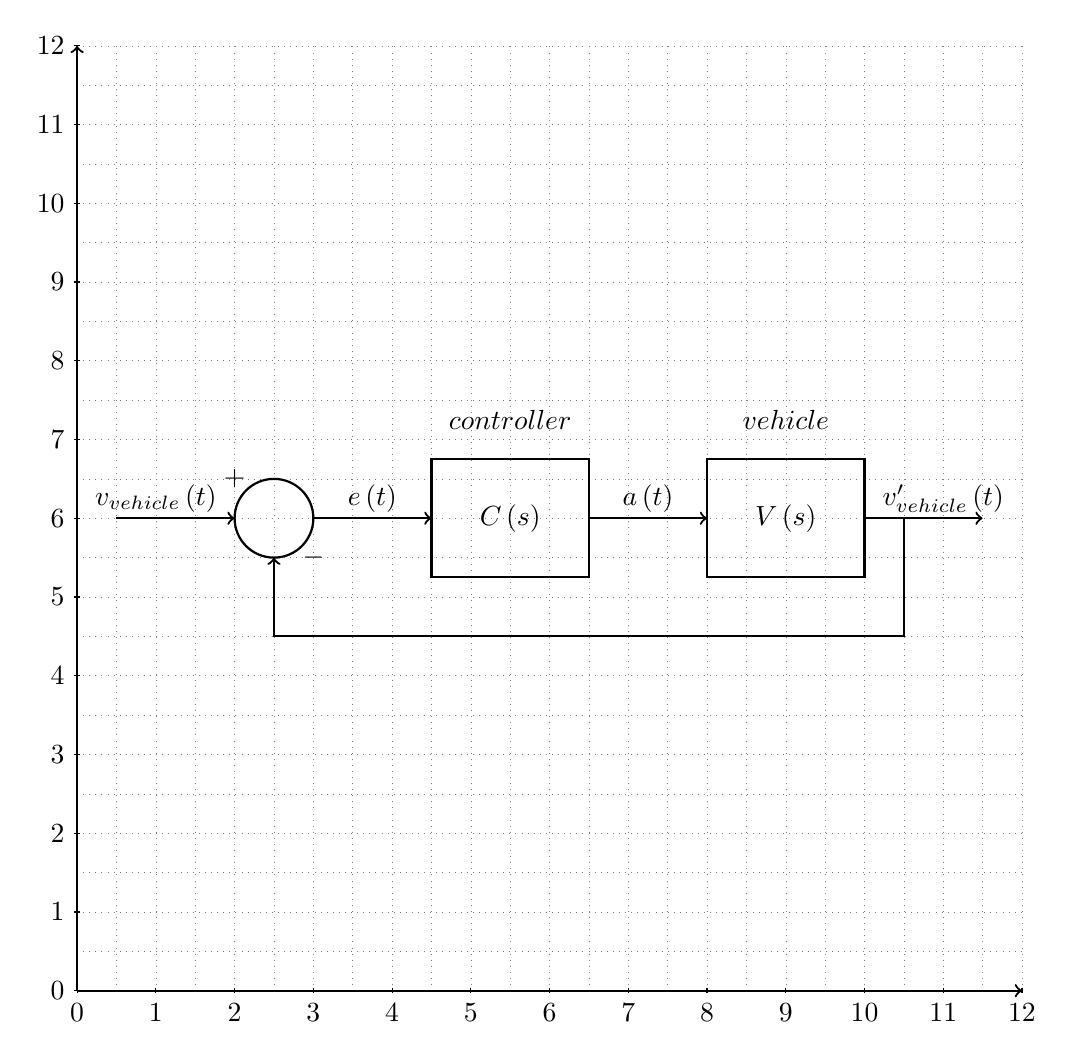
\begin{tikzpicture}
	 \draw[step = 0.5 cm, gray, very thin, dotted] (0, 0) grid (12, 12);
	 \draw[thick, ->] (0, 0) -- (12, 0);
	 \draw[thick, ->] (0, 0) -- (0, 12);
	 \foreach \x in {0, ..., 12}
	 \draw (\x cm, 1 pt) -- (\x cm, -1 pt) node[anchor = north] {$\x$};
	 \foreach \y in {0, ..., 12}
	 \draw (1 pt, \y cm) -- (-1 pt, \y cm) node[anchor = east] {$\y$};	
	 
	 \draw[thick, ->] (0.5, 6) -- (2, 6);
	 \node[align = center] at (1, 6.25) {$v_{vehicle}\left(t\right)$};	 
	 
	 \draw[thick] (2.5, 6) circle (0.5);
	 
	 \draw[thick, ->] (3, 6) -- (4.5, 6);
	 \node[align = center] at (3.75, 6.25) {$e\left(t\right)$};
	 
	 \draw[thick] (4.5, 6.75) rectangle (6.5, 5.25);
	 
	 \draw[thick, ->] (6.5, 6) -- (8, 6);
	 \node[align = center] at (7.25, 6.25) {$a\left(t\right)$};
	 
	 \draw[thick] (8, 6.75) rectangle (10, 5.25);
	 
	 \draw[thick, ->] (10, 6) -- (11.5, 6);
	 \node[align = center] at (11, 6.25) {$v_{vehicle}^{\prime}\left(t\right)$};
	 
	 \draw[thick, <-] (2.5, 5.5) -- (2.5, 4.5) -- (10.5, 4.5) -- (10.5, 6);
	 
	 \node[align = center] at (5.5, 6) {$C\left(s\right)$};
	 
	 \node[align = center] at (9, 6) {$V\left(s\right)$};
	 
	 \node[align = center] at (5.5, 7.25) {$controller$};
	 
	 \node[align = center] at (9, 7.25) {$vehicle$};
	 
	 \node[align = center] at (2, 6.5) {$+$};
	 
	 \node[align = center] at (3, 5.5) {$-$};
	 \end{tikzpicture}
	 
	 \begin{align}
	 Let &: e\left(t\right) = \left(v_{vehicle}^{\prime}\left(t\right) - v_{vehicle}\left(t\right)\right) \\
	 a\left(t\right) &= K_{p} e\left(t\right) + K_{i} \int e\left(t\right) dt + K_{d} \frac{de\left(t\right)}{dt}
	 \end{align}
	 
	 \begin{tikzpicture}
	 \draw[step = 0.5 cm, gray, very thin, dotted] (0, 0) grid (12, 12);
	 \draw[thick, ->] (0, 0) -- (12, 0);
	 \draw[thick, ->] (0, 0) -- (0, 12);
	 \foreach \x in {0, ..., 12}
	 \draw (\x cm, 1 pt) -- (\x cm, -1 pt) node[anchor = north] {$\x$};
	 \foreach \y in {0, ..., 12}
	 \draw (1 pt, \y cm) -- (-1 pt, \y cm) node[anchor = east] {$\y$};	
	 
	 \draw plot [smooth] coordinates {(2,0) (2.5,0.5) (3,1.5) (4, 4) (5.5, 5.25) (8, 5.5) (10, 5.5) (12, 5.5)};
	 \end{tikzpicture}
	 
	 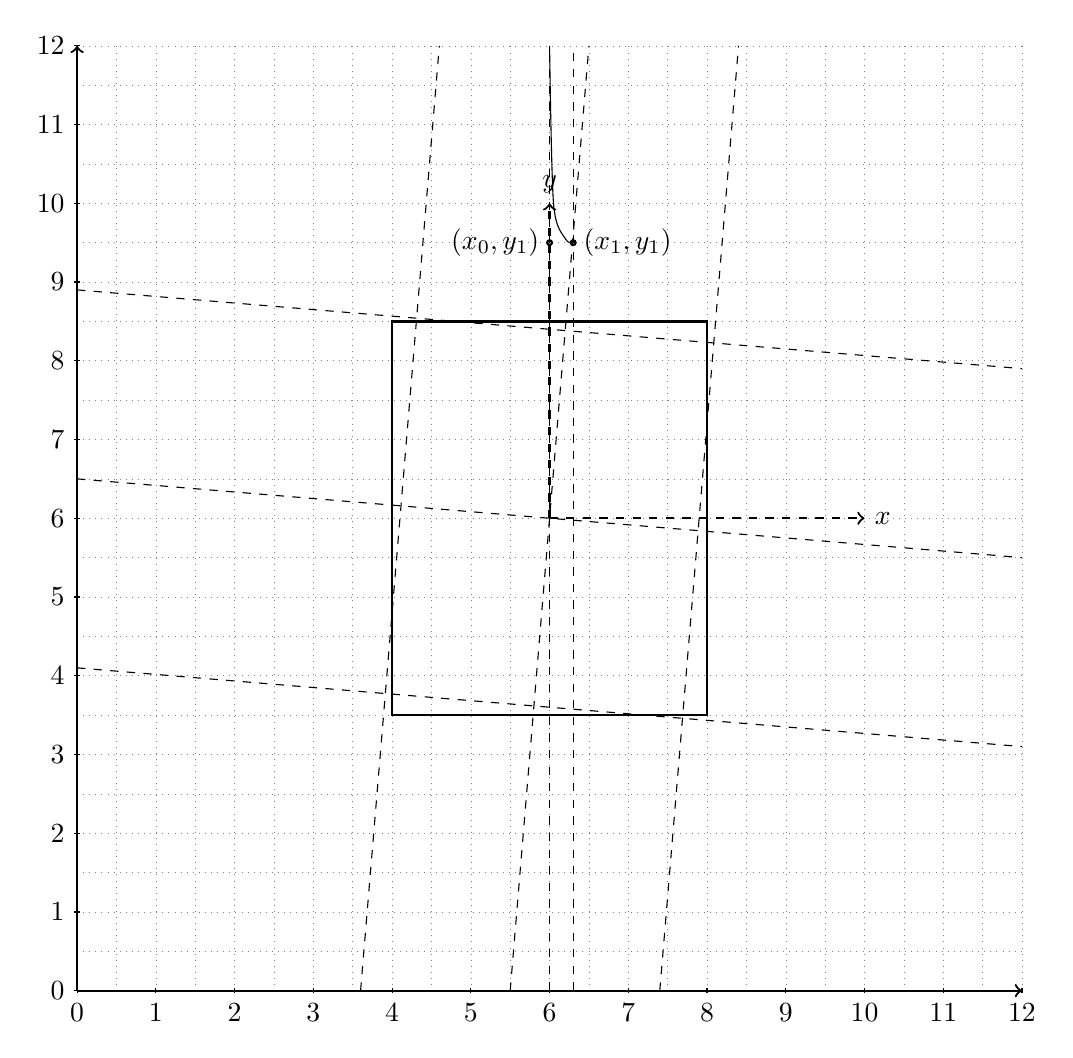
\begin{tikzpicture}
	 \draw[step = 0.5 cm, gray, very thin, dotted] (0, 0) grid (12, 12);
	 \draw[thick, ->] (0, 0) -- (12, 0);
	 \draw[thick, ->] (0, 0) -- (0, 12);
	 \foreach \x in {0, ..., 12}
	 \draw (\x cm, 1 pt) -- (\x cm, -1 pt) node[anchor = north] {$\x$};
	 \foreach \y in {0, ..., 12}
	 \draw (1 pt, \y cm) -- (-1 pt, \y cm) node[anchor = east] {$\y$};
	 
	 \draw[thick] (4, 8.5) rectangle (8, 3.5);
	 
	 \draw[thin, dashed] (6, 0) -- (6, 12);
	 \draw[thin, dashed] (5.5, 0) -- (6.5, 12);
	 
	 \draw[thin, dashed] (0, 6.5) -- (12, 5.5);
	 
	 \draw[thin, dashed] (3.6, 0) -- (4.6, 12);
	 \draw[thin, dashed] (7.4, 0) -- (8.4, 12);
	 
	 \draw[thin, dashed] (0, 4.1) -- (12, 3.1);
	 \draw[thin, dashed] (0, 8.9) -- (12, 7.9);
	 
	 \draw[thick, ->, dashed] (6, 6) -- (6, 10) node [anchor = south] {$y$};
	 
	 \draw[thick, ->, dashed] (6, 6) -- (10, 6) node [anchor = west] {$x$};
	 
	 \draw[thick] (6.3, 9.5) circle (0.03 cm) node [anchor = west] {$\left(x_{1}, y_{1}\right)$};
	 
	 \draw[thin, dashed] (6.3, 0) -- (6.3, 12);
	 
	 \draw[thick] (6, 9.5) circle (0.03 cm) node [anchor = east] {$\left(x_{0}, y_{1}\right)$};
	 
	 \draw plot [smooth] coordinates {(6.3,9.5) (6.2,9.55) (6.05,10) (6, 12)};
	 \end{tikzpicture}
	 
	 \begin{align}
	 Let &: e\left(t\right) = \left(x_{1} \left(t\right) - x_{0} \left(t\right)\right), x_{0} \left(t\right) = 0 \\
	 \implies e\left(t\right) &= x_{1} \left(t\right) \\
	 \theta \left(t\right) &= K_{p} e\left(t\right) + K_{i} \int e\left(t\right) dt + K_{d} \frac{de\left(t\right)}{dt} \\
	 \implies \theta \left(t\right) &= K_{p} x_{1}\left(t\right) + K_{i} \int_{0}^{x_{1}} x_{1}\left(t\right) dt + K_{d} \frac{dx_{1}\left(t\right)}{dt}
	 \end{align}
	 
	 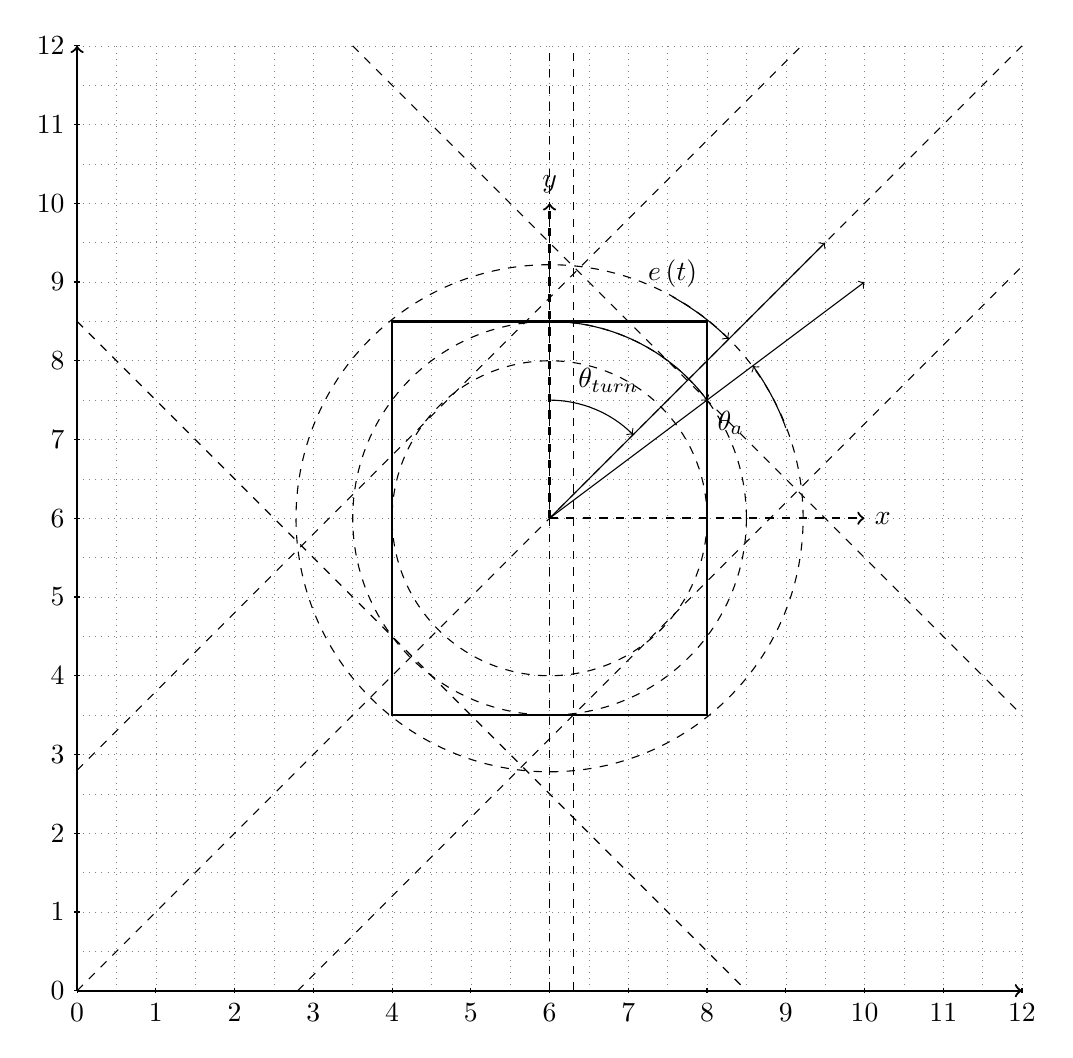
\begin{tikzpicture}
	 \draw[step = 0.5 cm, gray, very thin, dotted] (0, 0) grid (12, 12);
	 \draw[thick, ->] (0, 0) -- (12, 0);
	 \draw[thick, ->] (0, 0) -- (0, 12);
	 \foreach \x in {0, ..., 12}
	 \draw (\x cm, 1 pt) -- (\x cm, -1 pt) node[anchor = north] {$\x$};
	 \foreach \y in {0, ..., 12}
	 \draw (1 pt, \y cm) -- (-1 pt, \y cm) node[anchor = east] {$\y$};
	 
	 \draw[thick] (4, 8.5) rectangle (8, 3.5);
	 
	 \draw[thin, dashed] (6, 0) -- (6, 12);
	 \draw[thin, dashed] (0, 0) -- (12, 12);
	 
	 \draw[thick, ->, dashed] (6, 6) -- (6, 10) node [anchor = south] {$y$};
	 
	 \draw[thick, ->, dashed] (6, 6) -- (10, 6) node [anchor = west] {$x$};
	 
	 \draw[thin, dashed] (6.3, 0) -- (6.3, 12);
	 
	 \draw[thin, dashed] (6, 6) circle (3.22);
	 \draw[thin, dashed] (6, 6) circle (2.5);
	 \draw[thin, dashed] (6, 6) circle (2);
	 
	 \draw[thin, dashed] (3.5, 12) -- (12, 3.5); 
	 \draw[thin, dashed] (0, 8.5) -- (8.5, 0); 
	 \draw[thin, dashed] (2.8, 0) -- (12, 9.2);
	 \draw[thin, dashed] (0, 2.8) -- (9.2, 12);
	 
	 \draw[thin, ->] (6, 6) -- (9.5, 9.5);
	 
	 \draw[thin, ->] (6, 7.5) arc (90:45:1.5);
	 \node [align = center] at (6.75, 7.75) {$\theta_{turn}$};
	 
	 \draw[thin, ->] (6, 6) -- (10, 9);
	 \draw[thin, ->] (9, 7.15) arc (20:36:3.2);
	 \draw[thin, <-] (8.275, 8.275) arc (45:61:3.2) node [anchor = south] {$e\left(t\right)$};
	 
	 \draw[thin, ->] (6, 8.5) arc (90:36.5:2.5) node[anchor = north west] {$\theta_{a}$};
	 \end{tikzpicture}
	 
	 \begin{align}
	 Let &: e\left(t\right) = \left(\theta_{a} \left(t\right) - \theta_{turn} \left(t\right)\right) \\
	 \alpha \left(t\right) &= K_{p} e\left(t\right) + K_{i} \int e\left(t\right) dt + K_{d} \frac{de\left(t\right)}{dt}
	 \end{align}
	 
	 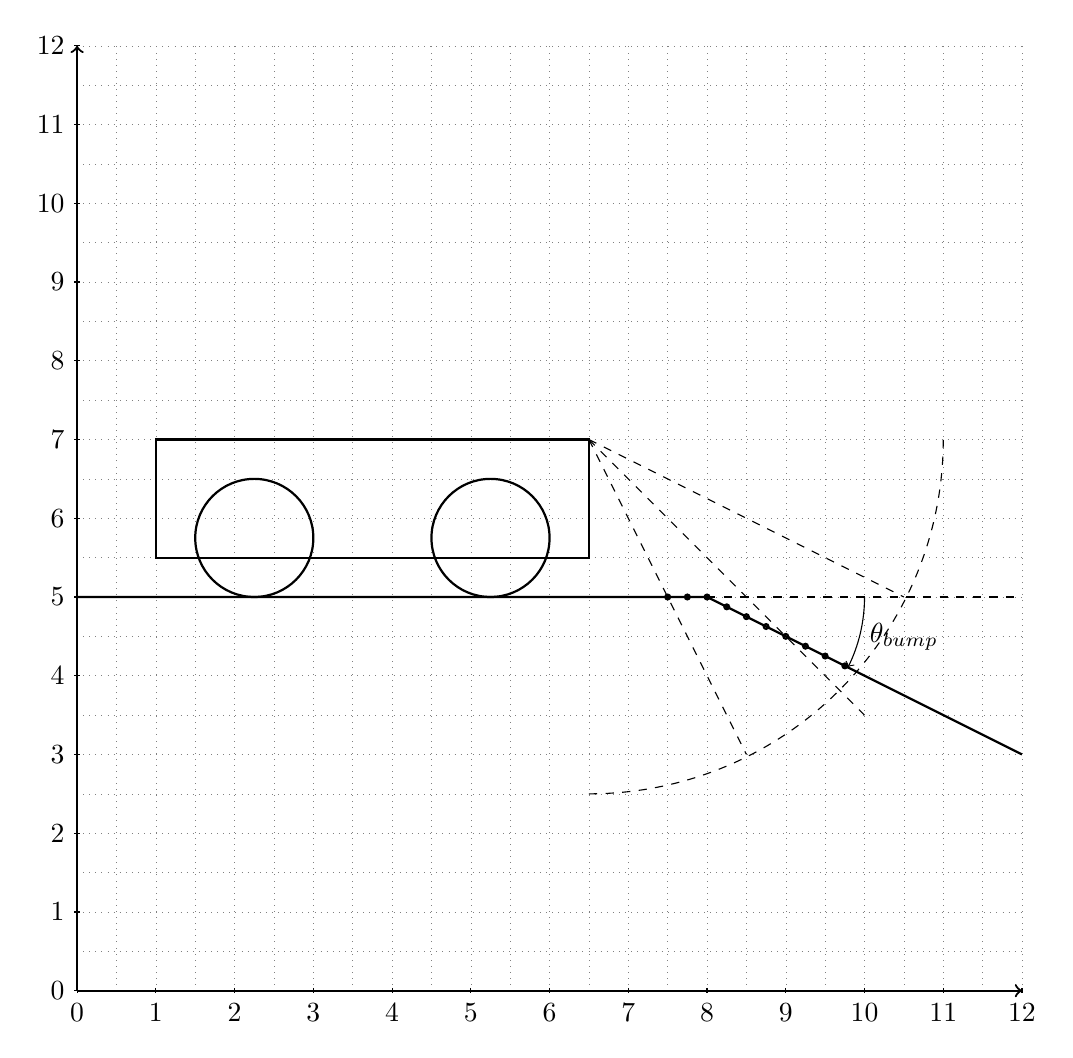
\begin{tikzpicture}
	 \draw[step = 0.5 cm, gray, very thin, dotted] (0, 0) grid (12, 12);
	 \draw[thick, ->] (0, 0) -- (12, 0);
	 \draw[thick, ->] (0, 0) -- (0, 12);
	 \foreach \x in {0, ..., 12}
	 \draw (\x cm, 1 pt) -- (\x cm, -1 pt) node[anchor = north] {$\x$};
	 \foreach \y in {0, ..., 12}
	 \draw (1 pt, \y cm) -- (-1 pt, \y cm) node[anchor = east] {$\y$};
	 
	 \draw [thick] (0, 5) -- (8, 5) -- (12, 3);
	 
	 \draw[thick] (1, 7) rectangle (6.5, 5.5);
	 
	 \draw[thick] (2.25, 5.75) circle (0.75);
	 \draw[thick] (5.25, 5.75) circle (0.75);
	 
	 \draw[thin, dashed] (6.5, 7) -- (8.5, 3);
	 \draw[thin, dashed] (6.5, 7) -- (10, 3.5);
	 \draw[thin, dashed] (6.5, 7) -- (10.5, 5);
	 
	 \draw[thin, dashed] (6.5, 2.5) arc (270:360:4.5);
	 
	 \draw[thick] (7.5, 5) circle (0.03 cm);
	 \draw[thick] (7.75, 5) circle (0.03 cm);
	 \draw[thick] (8, 5) circle (0.03 cm);
	 \draw[thick] (8.25, 4.875) circle (0.03 cm);
	 \draw[thick] (8.5, 4.75) circle (0.03 cm);
	 \draw[thick] (8.75, 4.625) circle (0.03 cm);
	 \draw[thick] (9, 4.5) circle (0.03 cm);
	 \draw[thick] (9.25, 4.375) circle (0.03 cm);
	 \draw[thick] (9.5, 4.25) circle (0.03 cm);
	 \draw[thick] (9.75, 4.125) circle (0.03 cm);
	 
	 \draw[thin, dashed] (8, 5) -- (12, 5);
	 
	 \draw[thin, ->] (10, 5) arc (0:-26.5:2);
	 
	 \node[align = center] at (10.5, 4.5) {$\theta_{bump}$};
	 \end{tikzpicture}
	 
	 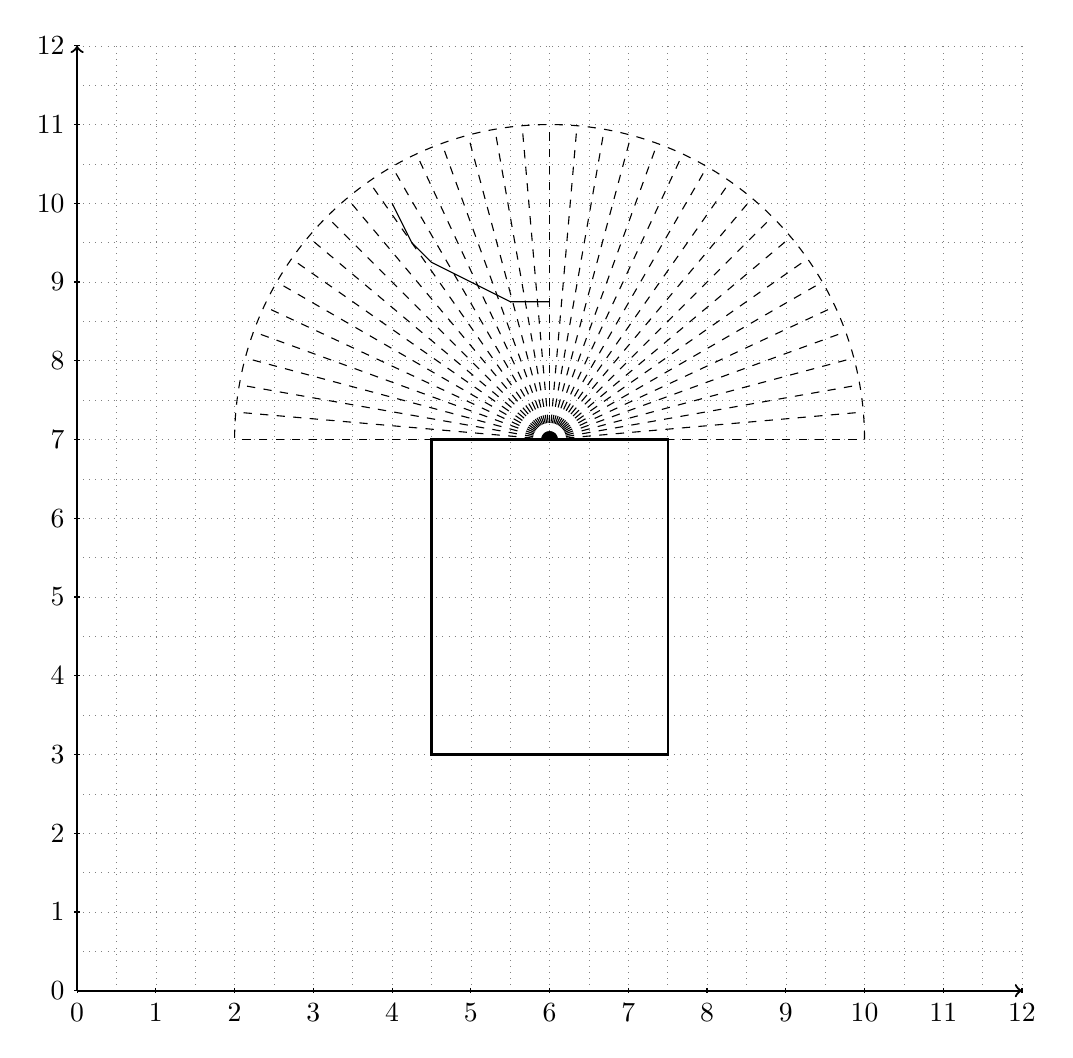
\begin{tikzpicture}
	 \draw[step = 0.5 cm, gray, very thin, dotted] (0, 0) grid (12, 12);
	 \draw[thick, ->] (0, 0) -- (12, 0);
	 \draw[thick, ->] (0, 0) -- (0, 12);
	 \foreach \x in {0, ..., 12}
	 \draw (\x cm, 1 pt) -- (\x cm, -1 pt) node[anchor = north] {$\x$};
	 \foreach \y in {0, ..., 12}
	 \draw (1 pt, \y cm) -- (-1 pt, \y cm) node[anchor = east] {$\y$};
	 
	 \draw[thick] (4.5, 7) rectangle (7.5, 3);
	 
	 \draw[thin, dashed] (10, 7) arc (0:180:4);
	 
	 \draw[thin, dashed] (6, 7) -- +(0:4);
	 \draw[thin, dashed] (6, 7) -- +(5:4); \draw[thin, dashed] (6, 7) -- +(10:4);
	 \draw[thin, dashed] (6, 7) -- +(15:4);
	 \draw[thin, dashed] (6, 7) -- +(20:4);
	 \draw[thin, dashed] (6, 7) -- +(25:4);
	 \draw[thin, dashed] (6, 7) -- +(30:4);
	 \draw[thin, dashed] (6, 7) -- +(35:4);
	 \draw[thin, dashed] (6, 7) -- +(40:4); \draw[thin, dashed] (6, 7) -- +(45:4);
	 \draw[thin, dashed] (6, 7) -- +(50:4);
	 \draw[thin, dashed] (6, 7) -- +(55:4);
	 \draw[thin, dashed] (6, 7) -- +(60:4);
	 \draw[thin, dashed] (6, 7) -- +(65:4);
	 \draw[thin, dashed] (6, 7) -- +(70:4);
	 \draw[thin, dashed] (6, 7) -- +(75:4); \draw[thin, dashed] (6, 7) -- +(80:4);
	 \draw[thin, dashed] (6, 7) -- +(85:4);
	 \draw[thin, dashed] (6, 7) -- +(90:4);
	 \draw[thin, dashed] (6, 7) -- +(95:4);
	 \draw[thin, dashed] (6, 7) -- +(100:4);
	 \draw[thin, dashed] (6, 7) -- +(105:4);
	 \draw[thin, dashed] (6, 7) -- +(110:4); \draw[thin, dashed] (6, 7) -- +(115:4);
	 \draw[thin, dashed] (6, 7) -- +(120:4);
	 \draw[thin, dashed] (6, 7) -- +(125:4);
	 \draw[thin, dashed] (6, 7) -- +(130:4);
	 \draw[thin, dashed] (6, 7) -- +(135:4);
	 \draw[thin, dashed] (6, 7) -- +(140:4);
	 \draw[thin, dashed] (6, 7) -- +(145:4);
	 \draw[thin, dashed] (6, 7) -- +(150:4);
	 \draw[thin, dashed] (6, 7) -- +(155:4); \draw[thin, dashed] (6, 7) -- +(160:4);
	 \draw[thin, dashed] (6, 7) -- +(165:4);
	 \draw[thin, dashed] (6, 7) -- +(170:4);
	 \draw[thin, dashed] (6, 7) -- +(175:4);
	 \draw[thin, dashed] (6, 7) -- +(180:4);
	 
	 \draw[thin] (4, 10) -- (4.25, 9.5) -- (4.5, 9.25) -- (5, 9) -- (5.5, 8.75) -- (6, 8.75);
	 \end{tikzpicture}
	 
	 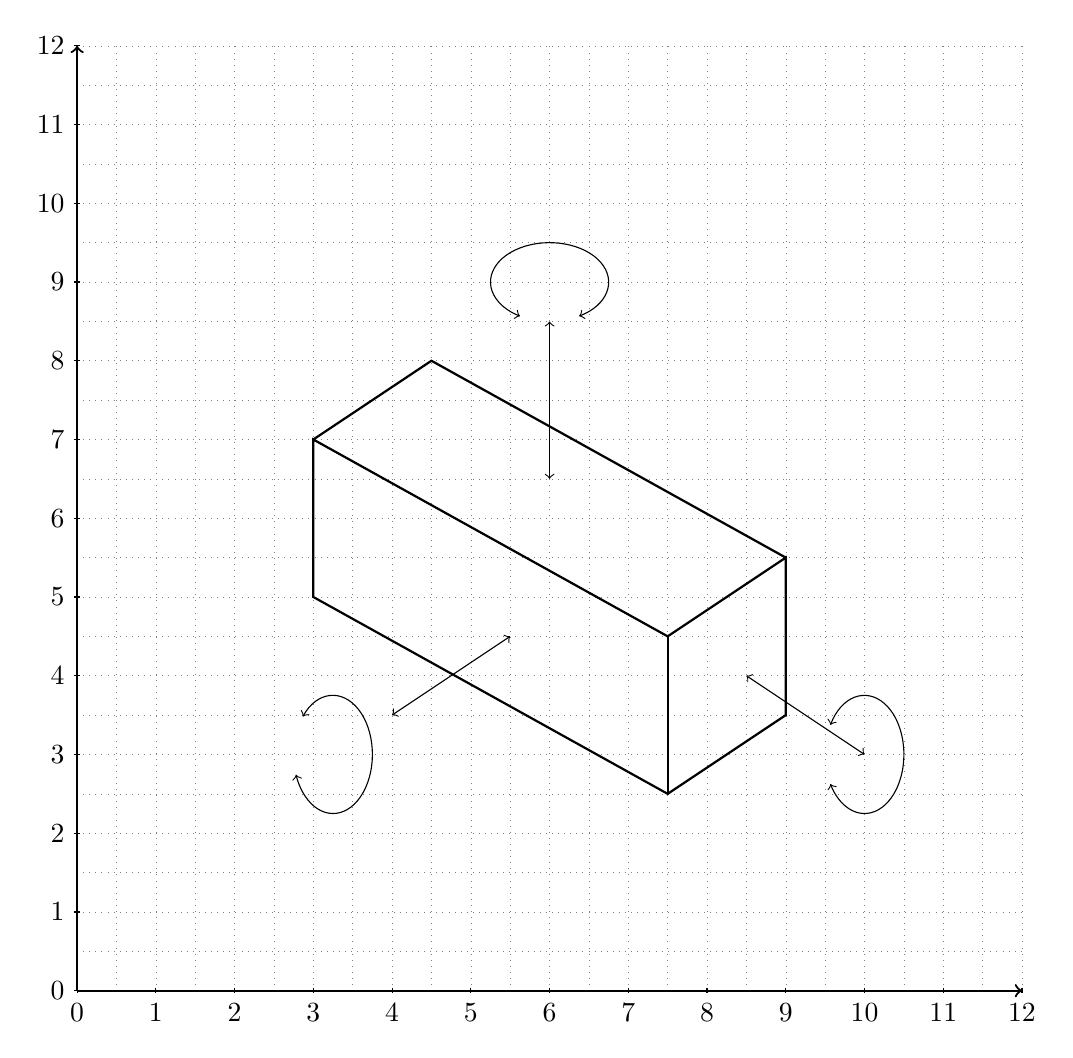
\begin{tikzpicture}
	 \tikzset{
	 	partial ellipse/.style args={#1:#2:#3}{
	 		insert path={+ (#1:#3) arc (#1:#2:#3)}
	 	}
	 }
 
	 \draw[step = 0.5 cm, gray, very thin, dotted] (0, 0) grid (12, 12);
	 \draw[thick, ->] (0, 0) -- (12, 0);
	 \draw[thick, ->] (0, 0) -- (0, 12);
	 \foreach \x in {0, ..., 12}
	 \draw (\x cm, 1 pt) -- (\x cm, -1 pt) node[anchor = north] {$\x$};
	 \foreach \y in {0, ..., 12}
	 \draw (1 pt, \y cm) -- (-1 pt, \y cm) node[anchor = east] {$\y$};
	 
	 \draw[thick] (3, 5) -- (7.5, 2.5) -- (9, 3.5) -- (9, 5.5) -- (7.5, 4.5) -- (3, 7) -- cycle;
	 \draw[thick] (3, 7) -- (4.5, 8) -- (9, 5.5);
	 \draw[thick] (7.5, 2.5) -- (7.5, 4.5);
	 
	 \draw[thin, <->] (6, 6.5) -- (6, 8.5);
	 \draw[thin, <->] (8.5, 4) -- (10, 3);
	 \draw[thin, <->] (4, 3.5) -- (5.5, 4.5);
 
	 \draw[thin, <->] (6, 9) [partial ellipse=-60:240:0.75 and 0.5];
	 \draw[thin, <->] (10, 3) [partial ellipse=150:-150:0.5 and 0.75];
	 \draw[thin, <->] (3.25, 3) [partial ellipse=140:-160:0.5 and 0.75];
	 \end{tikzpicture}
	 
	 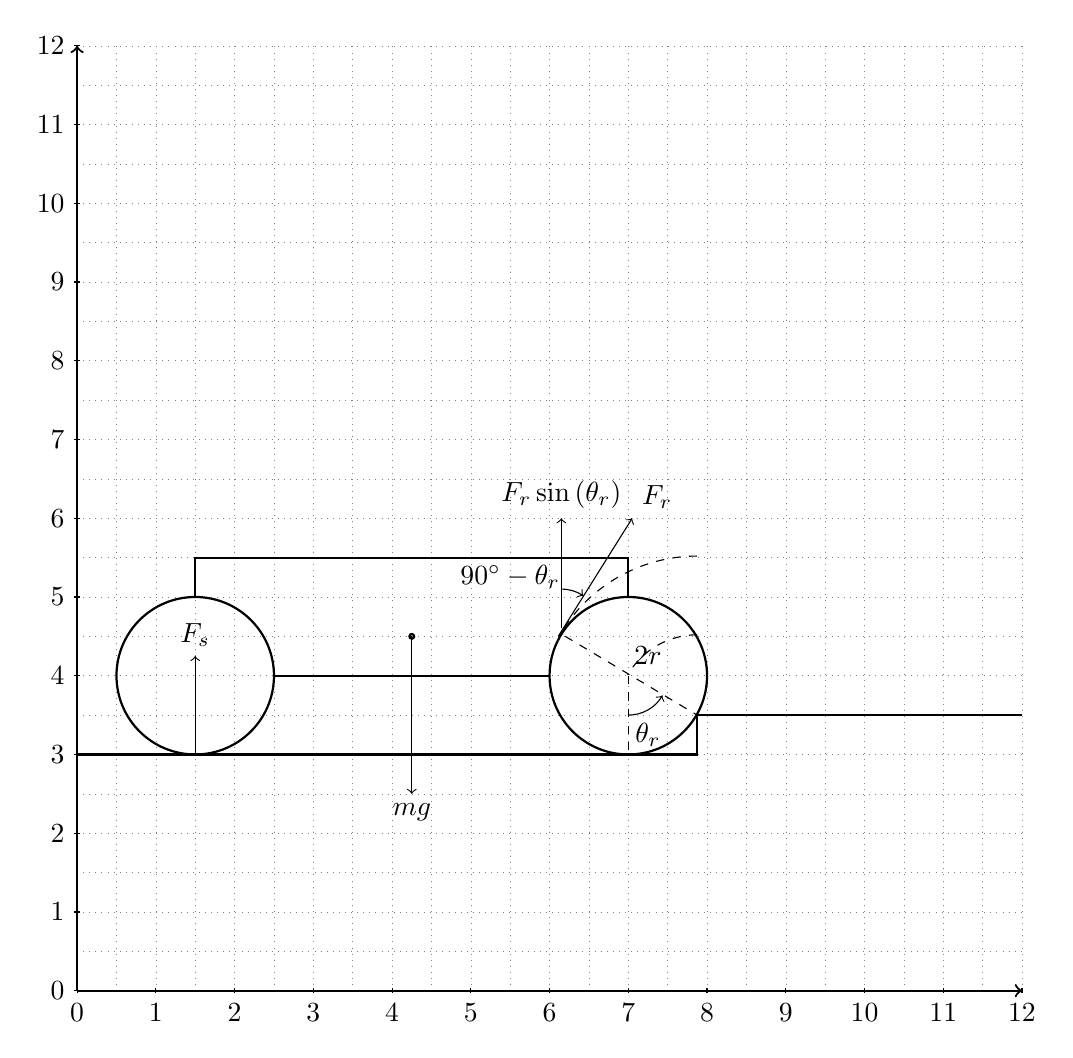
\begin{tikzpicture}
	 \draw[step = 0.5 cm, gray, very thin, dotted] (0, 0) grid (12, 12);
	 \draw[thick, ->] (0, 0) -- (12, 0);
	 \draw[thick, ->] (0, 0) -- (0, 12);
	 \foreach \x in {0, ..., 12}
	 \draw (\x cm, 1 pt) -- (\x cm, -1 pt) node[anchor = north] {$\x$};
	 \foreach \y in {0, ..., 12}
	 \draw (1 pt, \y cm) -- (-1 pt, \y cm) node[anchor = east] {$\y$};
	 
	 \draw[thick] (0, 3) -- (7.875, 3) -- (7.875, 3.5) -- (12, 3.5);
	 
	 \draw[thick] (7, 4) circle (1);
	 \draw[thick] (1.5, 4) circle (1);
	 
	 \draw[thick] (2.5, 4) -- (6, 4);
	 \draw[thick] (1.5, 5) -- (1.5, 5.5) -- (7, 5.5) -- (7, 5);
	 
	 \draw[thin, ->] (4.25, 4.5) -- (4.25, 2.5) node[anchor = north] {$m g$};
	 
	 \draw[thin, dashed] (6.2, 4.5) -- (7.875, 3.5);
	 
	 \draw[thin, ->] (6.11, 4.5) -- (7.05, 6) node[anchor = south west] {$F_{r}$};
	 
	 \node[align = center] at (7.25, 4.25) {$2 r$};
	 
	 \draw[thick] (4.25, 4.5) circle (0.03 cm);
	 
	 \draw[thin, dashed] (7, 4) -- (7, 3);
	 \draw[thin, ->] (1.5, 3) -- (1.5, 4.25) node[anchor = south] {$F_{s}$};
	 
	 \draw[thin, ->] (7, 3.5) arc (270:330:0.5);
	 
	 \node[align = center] at (7.25, 3.25) {$\theta_{r}$};
	 
	 \draw[thin, ->] (6.15, 4.6) -- (6.15, 6) node [anchor = south] {$F_{r} \sin \left(\theta_{r}\right)$};
	 
	 \draw[thin, ->] (6.15, 5.1) arc (90:56:0.5);
	 
	 \node[align = center] at (5.5, 5.25) {$90^{\circ} - \theta_{r}$};
	 
	 \draw[thin, dashed] (7.875, 5.52) arc (90:150:2.02);
	 
	 \draw[thin, dashed] (7.875, 4.52) arc (90:150:1.02);
	 \end{tikzpicture}
	 
	 \begin{align}
	 mg &= F_{s} + F_r \sin \left(\theta_{r}\right) \\
	 \implies F_{s} &= mg - F_r \sin \left(\theta_{r}\right) \\
	 F_{s} \times \left(l + r \sin \left(\theta_{r}\right)\right) + F_{r} \times 2 r &= mg \times \left(\frac{l}{2} + r \sin \left(\theta_{r}\right)\right) \\
	 \implies \left(mg - F_r \sin \left(\theta_{r}\right)\right) \times \left(l + r \sin \left(\theta_{r}\right)\right) + F_{r} \times 2 r &= mg \times \left(\frac{l}{2} + r \sin \left(\theta_{r}\right)\right) \\
	 \implies mg \times \left(l + r \sin \left(\theta_{r}\right)\right) - F_r \sin \left(\theta_{r}\right) \times \left(l + r \sin \left(\theta_{r}\right)\right) + F_{r} \times 2 r &= mg \times \left(\frac{l}{2} + r \sin \left(\theta_{r}\right)\right) \\
	 \implies mg \times \left(l + r \sin \left(\theta_{r}\right)\right) - mg \times \left(\frac{l}{2} + r \sin \left(\theta_{r}\right)\right) &= F_r \sin \left(\theta_{r}\right) \times \left(l + r \sin \left(\theta_{r}\right)\right) - F_{r} \times 2 r \\
	 \implies mg \times \frac{l}{2} &= F_{r} \left(\sin \left(\theta_{r}\right) \times \left(l + r \sin \left(\theta_{r}\right)\right) - 2 \times r\right) \\
	 \implies mg \times \frac{l}{2} &= F_{r} \left(l \sin \left(\theta_{r}\right) + r \sin^{2} \left(\theta_{r}\right) - 2 r\right) \\
	 \implies F_{r} &= \frac{mgl}{2 \left(l \sin \left(\theta_{r}\right) + r \sin^{2} \left(\theta_{r}\right) - 2 r\right)} \\
	 \tau &= F_{r} \times 2 r \\
	 \implies \tau &= 2 F_{r} r
	 \end{align}
	 
	 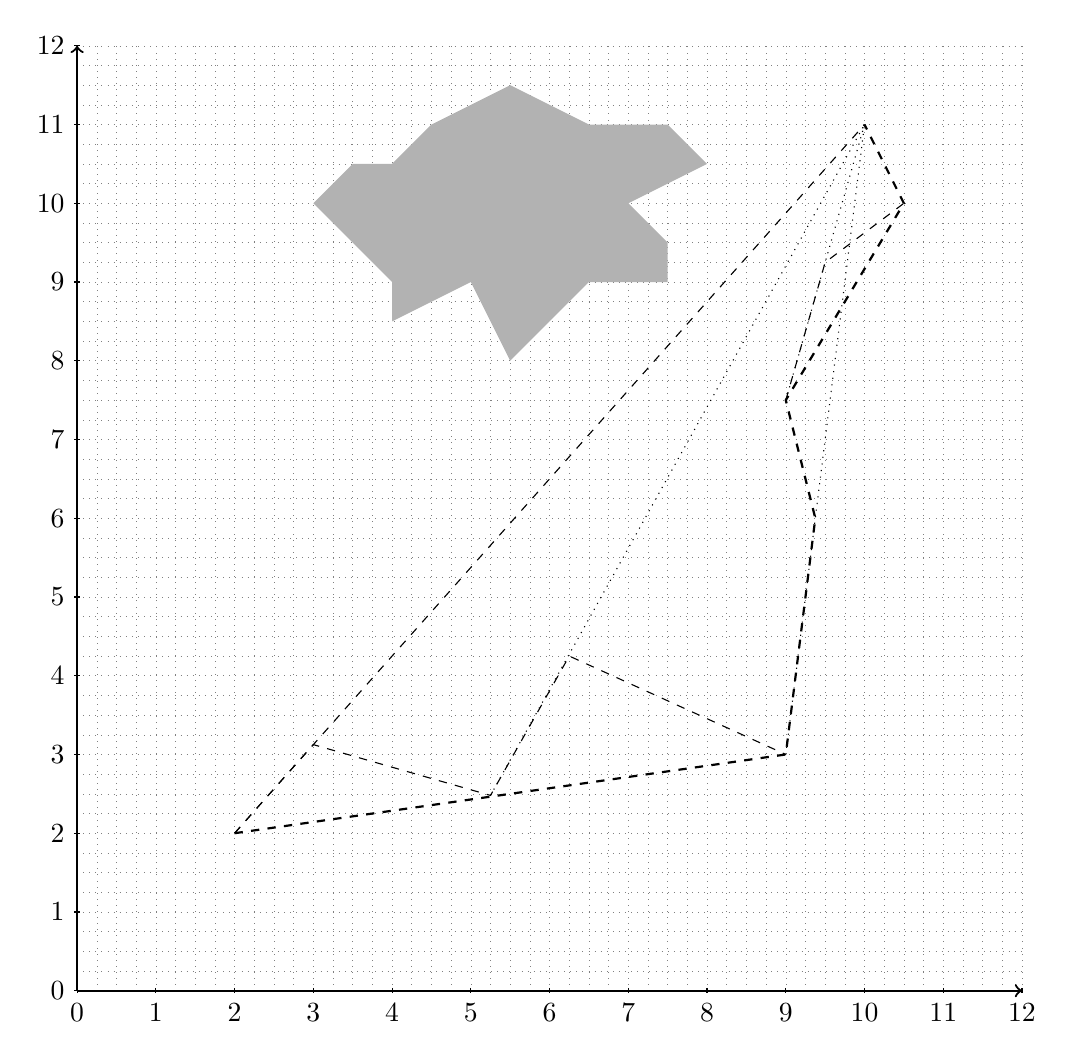
\begin{tikzpicture}	 
	 \draw[step = 0.25 cm, gray, very thin, dotted] (0, 0) grid (12, 12);
	 \draw[thick, ->] (0, 0) -- (12, 0);
	 \draw[thick, ->] (0, 0) -- (0, 12);
	 \foreach \x in {0, ..., 12}
	 \draw (\x cm, 1 pt) -- (\x cm, -1 pt) node[anchor = north] {$\x$};
	 \foreach \y in {0, ..., 12}
	 \draw (1 pt, \y cm) -- (-1 pt, \y cm) node[anchor = east] {$\y$};	
	 
	 \fill[black!30!white] (4, 8.5) -- (5, 9) -- (5.5, 8) -- (6, 8.5) -- (6.5, 9) -- (7.5, 9) -- (7.5, 9.5) -- (7, 10) -- (8, 10.5) -- (7.5, 11) -- (6.5, 11) -- (5.5, 11.5) -- (4.5, 11) -- (4, 10.5) -- (3.5, 10.5) -- (3, 10) -- (3.5, 9.5) -- (4, 9) -- cycle;
	 
	 \draw[thin, dashed] (2, 2) -- (10, 11);
	 
	 \draw[thin, dotted] (5.25, 2.48) -- (10, 11);
	 \draw[thin, dotted] (9, 3) -- (10, 11);
	 \draw[thin, dotted] (9, 7.5) -- (10, 11);
	 
	 \draw[thin, dashed] (2, 2) -- (3, 3.125) -- (5.25, 2.48) -- (6.25, 4.25) -- (9, 3);
	 \draw[thin, dashed] (9, 7.5) -- (9.5, 9.25) -- (10.5, 10);
	 \draw[thick, dashed] (2, 2) -- (9, 3) -- (9.375, 6) -- (9, 7.5) -- (10.5, 10) -- (10, 11);
	 \end{tikzpicture}
\end{document}